\documentclass[12pt]{article}\usepackage[]{graphicx}\usepackage[]{color}
%% maxwidth is the original width if it is less than linewidth
%% otherwise use linewidth (to make sure the graphics do not exceed the margin)
\makeatletter
\def\maxwidth{ %
  \ifdim\Gin@nat@width>\linewidth
    \linewidth
  \else
    \Gin@nat@width
  \fi
}
\makeatother

\definecolor{fgcolor}{rgb}{0.345, 0.345, 0.345}
\newcommand{\hlnum}[1]{\textcolor[rgb]{0.686,0.059,0.569}{#1}}%
\newcommand{\hlstr}[1]{\textcolor[rgb]{0.192,0.494,0.8}{#1}}%
\newcommand{\hlcom}[1]{\textcolor[rgb]{0.678,0.584,0.686}{\textit{#1}}}%
\newcommand{\hlopt}[1]{\textcolor[rgb]{0,0,0}{#1}}%
\newcommand{\hlstd}[1]{\textcolor[rgb]{0.345,0.345,0.345}{#1}}%
\newcommand{\hlkwa}[1]{\textcolor[rgb]{0.161,0.373,0.58}{\textbf{#1}}}%
\newcommand{\hlkwb}[1]{\textcolor[rgb]{0.69,0.353,0.396}{#1}}%
\newcommand{\hlkwc}[1]{\textcolor[rgb]{0.333,0.667,0.333}{#1}}%
\newcommand{\hlkwd}[1]{\textcolor[rgb]{0.737,0.353,0.396}{\textbf{#1}}}%

\usepackage{framed}
\makeatletter
\newenvironment{kframe}{%
 \def\at@end@of@kframe{}%
 \ifinner\ifhmode%
  \def\at@end@of@kframe{\end{minipage}}%
  \begin{minipage}{\columnwidth}%
 \fi\fi%
 \def\FrameCommand##1{\hskip\@totalleftmargin \hskip-\fboxsep
 \colorbox{shadecolor}{##1}\hskip-\fboxsep
     % There is no \\@totalrightmargin, so:
     \hskip-\linewidth \hskip-\@totalleftmargin \hskip\columnwidth}%
 \MakeFramed {\advance\hsize-\width
   \@totalleftmargin\z@ \linewidth\hsize
   \@setminipage}}%
 {\par\unskip\endMakeFramed%
 \at@end@of@kframe}
\makeatother

\definecolor{shadecolor}{rgb}{.97, .97, .97}
\definecolor{messagecolor}{rgb}{0, 0, 0}
\definecolor{warningcolor}{rgb}{1, 0, 1}
\definecolor{errorcolor}{rgb}{1, 0, 0}
\newenvironment{knitrout}{}{} % an empty environment to be redefined in TeX

\usepackage{alltt}

\usepackage{sbc-template}

\usepackage{tensor}
\usepackage{natbib}
\usepackage{booktabs}
\usepackage{xspace}
\usepackage{placeins}
\usepackage{hyperref}
\usepackage{mathtools}
\usepackage{courier} % Required for the courier font

\usepackage{fancyhdr} % Required for custom headers
\usepackage{lastpage} % Required to determine the last page for the footer
\usepackage{extramarks} % Required for headers and footers
\usepackage{graphicx} % Required to insert images
\usepackage{listings} % Required for insertion of code
\usepackage{courier} % Required for the courier font
\usepackage{lipsum} % Used for inserting dummy 'Lorem ipsum' text into the template
\usepackage[usenames,dvipsnames,svgnames,table]{xcolor}
\usepackage{hyperref}
\usepackage{float}


\title{Working Specifications for Initial Measurements Under \\
      ESHB 1774 and SSHB 1566}

\author{Joseph Mienko\inst{1}}

\address{Partners for Our Children, School of Social Work\\
  University of Washington, Seattle, Washington}
\IfFileExists{upquote.sty}{\usepackage{upquote}}{}


\begin{document}

\definecolor{shadecolor}{rgb}{0.969, 0.969, 0.969}

\definecolor{sqlred}{rgb}{0.6,0,0} % for strings
\definecolor{sqlgreen}{rgb}{0.25,0.5,0.35} % comments
\definecolor{sqlpurple}{rgb}{0.5,0,0.35} % keywords
\definecolor{sqlblue}{rgb}{0.25,0.35,0.75} % docs
 

\lstset{basicstyle=\ttfamily\small
        ,keywordstyle=\color{sqlblue}\bfseries
        ,stringstyle=\color{red}
        ,commentstyle=\color{sqlgreen}
        ,backgroundcolor=\color{shadecolor}
        ,xleftmargin=-3pt
        ,xrightmargin=-3pt
        ,tabsize=2
        ,numbersep=5pt} 
        

%\SweaveOpts{concordance=TRUE}

%\definecolor{shadecolor}{rgb}{0.969, 0.969, 0.969}
%\definecolor{sqlred}{rgb}{0.6,0,0} % for strings
%\definecolor{sqlgreen}{rgb}{0.25,0.5,0.35} % comments
%\definecolor{sqlpurple}{rgb}{0.5,0,0.35} % keywords
%\definecolor{sqlblue}{rgb}{0.25,0.35,0.75} % docs
   
\maketitle

\section{Safety}
\subsection{Safety Concerns}
\subsubsection{Incidence Rate of Referrals ($IRR$)}

The incidence of reports of household safety concerns ($IRR$) shall be defined as the total number of first referrals to Children's Administration (CA) per month, per 1,000 households with own children under the age of 18 as defined by the US Census. This measure will focus only on those referrals aledging child maltreatment or an eminent risk of serious harm to the child. This rate shall be calculated simply by 
\begin{equation}\label{eq:IRR}
IRR = (I_R \div P_{H<18}) \cdot 1,000
\end{equation}
where $I_R$ represents the total number of first referrals occuring during the month and $P_{H<18}$ the number of households with own children under the age of 18 as defined by the US Census. To the extent that estimates are available, values of $P_{H<18}$ (and subsequent measures of the general population used in this document) shall be calculated from the following sources in order of priority:

\begin{enumerate}
  \item US Census,
  \item American Community Survey (ACS), 
  \item Office of Financial Management (OFM), and 
  \item Linear interpolation taking the above estimates as ``True'' values. 
\end{enumerate}

\subsubsection{Finding Rate ($FR$)}

The rate of household findings ($FR$) shall be defined as the monthly total number of first findings of child-abuse or neglect per 1,000 referrals to CA with no prior history of a founded allegation of child abuse or neglect. This measure will focus only on those referrals aledging child maltreatment or an eminent risk of serious harm to the child and will be calculated at the household level. A household is considered to have a finding if any allegation from a given referral is founded. This rate shall be calculated as 
\begin{equation}\label{eq:FR}
FR = (F \div I_{R_{NPF}}) \cdot 1,000
\end{equation}
where $F$ represents the total findings occuring during the month among referrals for households with no previous finding ($I_{R_{NPF}}$). 


\subsection{Recurrence of Safety Concerns}

\subsubsection{Second-Order Rereferral Rate ($RRR_2$)}

In measuring rereferrals, it is important to distinguish between first referrals ($IR_S$) and rereferrals. In general, those households that experience at least one referral to the child welfare system are at an increased risk of rereferral. As such, there is interest in distinguishing between first and higher order referrals (e.g. second referrals, third referrals, etc.). 

The order-specific rereferral rate is defined as the number of referrals of a given order during a month per 1,000 households with own children under the age of 18. The formula for the first referral is given in formula ~\ref{eq:IRR}. The formula for $ith$ order rereferral rates is 
\begin{equation}\label{eq:RRRi}
RRR_i = \frac{I_{R_i}}{P_{i-1PR<18}} \cdot 1,000
\end{equation}
where $I_{R_i}$ represents the total number of $ith$ order rereferrals and $P_{i-1PR<18}$ represents the number of $ith-1$ order referrals in which all children in the household are still under the age of 18. At this time, it is proposed that only second-order rereferrals ($RRR_2$) be used as measures under 1774. Future reports may include higher-order rereferrals. 

\subsubsection{Second-Order Refinding Rate ($RFR_2$)}

Similarly to rereferrals, those households that experience at least one finding ($FR$) to the child welfare system are at an increased risk of refinding. As such, there is interest in distinguishing between first and higher order referrals (e.g. second referrals, third referrals, etc.). 

The order-specific refinding rate is defined as the number of findings of a given order during a month per 1,000 households with own children under the age of 18 who have received $i-1$ prior referrals. The formula for the first referral is given in formula ~\ref{eq:FR}. The formula for $ith$ order rereferral rates is 
\begin{equation}\label{eq:RRRi}
RFR_i = \frac{I_{F_i}}{P_{i-1PF<18}} \cdot 1,000
\end{equation}
where $I_{F_i}$ represents the total number of $ith$ order refindings and $P_{i-1PF<18}$ represents the number of $ith-1$ order findings in which all children in the household are still under the age of 18. As with rereferrals, it is proposed that only second-order refindings ($RFR_2$) be used as measures under 1774. Future reports may include higher-order refindings. 

\subsection{Placement in Out-Of-Home Care}

\subsubsection{Incidence Rate of Placement ($IRP$)}

The incidence of placement into out-of-home care ($IRP$) shall be defined as the monthly total number of referrals to Children's Administration per 1,000 persons under the age of 18. This rate shall be calculated simply by 
\begin{equation}\label{eq:IRP}
IRP = (I_P \div P_C) \cdot 1,000
\end{equation}
where $I_P$ represents the total number of placements occuring during the month and $P_C$ the number of children under the age of 18 in the general population. To the extent that estimates are available, values of $P_C$ shall be calculated from the same sources and order of priority as in $P_H$ above.

\subsubsection{Placement Rate ($PR$)}

The rate of placement ($PR$) shall be defined as the monthly total number of first placements per 1,000 referrals to CA with no prior history of a placement in the household. For consistency with previous measurements, this measure will focus only on those referrals aledging child maltreatment or an eminent risk of serious harm to the child and will be calculated at the household level. A household is considered to have a placement if any child associated with the home on a given referral is placed into out-of-home care. This rate shall be calculated as 
\begin{equation}\label{eq:PR}
PR = (P \div I_{R_{NPP}}) \cdot 1,000
\end{equation}
where $P$ represents the total placements occuring during the month among referrals for households with no previous placement ($I_{R_{NPP}}$). 

\subsection{Maltreatment in Foster Care}

\subsubsection{Foster Care Finding Rate (${}_{FC}FR$)}

The final safety measurement concerns the rate of findings per day of foster care. This is the first ``care-day'' measurement proposed in this document - measurements in which the denominator is a count of days of out-of-home care for some population as opposed to a count of some type of person. 
The Foster-Care Finding Rate (${}_{FC}FR$) follows the similarly named proposed CFSR measurement where ${}_{FC}FR$ is defined as 
\begin{equation}\label{eq:_FCFR}
{}_{FC}FR = \frac{{}_{FC}I_F}{c} \cdot 100,000
\end{equation}
where $c$ represents the total number of care days provided by CA in a given year and ${}_{FC}I_F$ represents the number of maltreatment findings for children in out-of-home care over that period. This measurement excludes children in foster care for less than 8 days and also excludes reports made within the first 7 days of the referral. 

\section{Permanency}

\subsection{Time to Permanence}

\subsubsection{Percentage of Children Remaining in Care After 1 Year (${}_{P}\hat{S}(365)$)}

This measurement is similar to the proposed CFSR measurement requiring exit to permanency within 12 months. However, instead of calculating a specific percentage, we propose that a Kaplan-Meier estimator be used to better account for right censoring of children who either age-out of the system or exit to a form of permanency other than adoption, reunification, or some form of guardianship. 
 
The Kaplan-Meier estimator for a federally recognized form of permanency $P$ is given as
\begin{equation}\label{eq:KM1}
{}_P\hat S(t) = \prod\limits_{t_i<t} \frac{n_i-p_{i}}{n_i}
\end{equation}
where $n_{i}$ is the number of children entering out-of-home care in a given fiscal year who are still in care just prior to time $t_{i}$, and $p_{i}$ is the number of permanency events at $t_{i}$. Thus, the probability of exit within 1 year is given as ${}_P\hat S(365)$. A reasonable approximation of the new CFSR measurement is given as $(1 - {}_P\hat S(365)) \cdot 100$. For the sake of simplicity, we propose simply reporting annual calculations of ${}_{P}\hat{S}(365)$ for this measure. All children who stay in care for less than 8 days will be excluded from this measurement. Children aging out of care or experiencing a permanency outcome other than reunification, adoption, or some form of guardianship will be treated as right-censored to observation. 

\subsubsection{Percentage of Legally Free Children Awaiting Adoption After 1 Year (${}_{A}\hat{S}(365)$)}

This measurement will also make use of a Kaplan-Meier estimator. Specifically, the Kaplan-Meier estimator for adoption $A$ is given as
\begin{equation}\label{eq:KM}
{}_A\hat S(t) = \prod\limits_{t_i<t} \frac{n_i-a_{i}}{n_i}
\end{equation}
where $n_{i}$ is the number of children entering legally-free status in a given fiscal year who have not yet been adopted just prior to time $t_{i}$, and $a_{i}$ is the number of adoption events at $t_{i}$. Thus, the probability of adoption within 1 year is given as ${}_A\hat S(365)$. Children aging out of care or experiencing a permanency outcome other than adoption will be treated as right-censored to observation. 

\subsection{Duration of Permanence}

\subsubsection{Percentage of Children Reentering Care Within 1 Year (${}_{R}\hat{S}(365)$)}

This measurement will also make use of a Kaplan-Meier estimator. Specifically, the Kaplan-Meier estimator for reentry $R$ is given as
\begin{equation}\label{eq:KM}
{}_R\hat S(t) = \prod\limits_{t_i<t} \frac{n_i-r_{i}}{n_i}
\end{equation}
where $n_{i}$ is the number of children entering permanency in a given fiscal year who have not yet reentered care just prior to time $t_{i}$, and $r_{i}$ is the number of reentry events at $t_{i}$. Thus, the probability of reentry within 1 year is given as ${}_R\hat S(365)$. Children aging out of care or experiencing a permanency outcome other than adoption will be treated as right-censored to observation. Children who stay in care for less than 8 days will be excluded from this measurement.

\subsection{Placement Mobility}

\subsubsection{Duration-specific mobility rate ($M^d$)}
This measurement will adopt the basic approach of the analagous proposed CFSR measurement in which total placements are measured against the number of care days experienced for children during their first year of care. In this measurement, we propose that we extend this basic logic to a duration-specific mobility measurement in which a care-day mobility rate is calculated for the first through tenth duration periods ($d$) of care such that $M^d$ is given as 
\begin{equation}\label{eq:M_d}
M^d = (m^d \div C^d) \cdot 100,000
\end{equation}
where $m^d$ is the count of placement moves during the $dth$ year and $C^d$ is the number of care days associated with the $dth$ year. Children who stay in care for less than 8 days in their original placement episode will be excluded from this measurement.

\subsubsection{Transition-Duration-Specific mobility rate (${}_tM^d$)}
In order to get a sense of the \emph{types} of transitions that are experienced by children, $M^d$ shall be extended to also measure the type of transition that children are moving toward ($t$) (i.e. foster care ($f$), relative placement ($r$), and group care ($g$.). The ${}_tM^d$ measurement shall be calculated identically to $M_d$ above. However, ${}_tM^d$ shall be calculated seperately for $t=f$, $t=r$, and $t=g$. 

\subsubsection{Age-order-specific AWOL rate ($A^i_d$)}
This measurement will adopt the basic approach of the analagous proposed CFSR measurement in which total placements are measured against the number of care days experienced for children during their first year of care. In this measurement, we propose that we extend this basic logic to a duration-specific mobility measurement in which a care-day mobility rate is calculated for the first through tenth duration periods ($d$) of care such that $M^d$ is given as 
\begin{equation}\label{eq:M_d}
M^d = (m^d \div C^d) \cdot 100,000
\end{equation}
where $m^d$ is the count of placement moves during the $dth$ year and $C^d$ is the number of care days associated with the $dth$ year. Children who stay in care for less than 8 days in their original placement episode will be excluded from this measurement.


\section{Well-Being}

\subsection{Maintenance of Family Relationships}

\subsection{Educational Readiness}

\subsection{Adult Functioning}


\subsubsection{Incidence of reports of safety concerns}

\paragraph{The incidence of reports of household safety concerns}

\subparagraph{Definition} The incidence of reports of household safety concerns ($IR_R$) shall be defined as the total number of first referrals to Children's Administration (CA) per month, per 1,000 households with own children under the age of 18 as defined by the US Census. This measure will focus only on those referrals aledging child maltreatment or an eminent risk of serious harm to the child. This rate shall be calculated simply by 

\begin{equation}\label{eq:IRR}
IR_R = (I_R \div P_{H<18}) \cdot 1,000
\end{equation}

where $I_R$ represents the total number of first referrals occuring during the month and $P_{H<18}$ the number of households with own children under the age of 18 as defined by the US census. To the extent that estimates are available, values of $P_{H<18}$ shall be calculated from the following sources in order of priority:

\begin{enumerate}
  \item US Census,
  \item American Community Survey (ACS), 
  \item Office of Financial Management (OFM), and 
  \item Linear interpolation taking the above estimates as ``True'' values. 
\end{enumerate}

\subparagraph{SQL Code}

The SQL code used to obtain data for this measurement is as follows: 

\lstinputlisting[language=SQL]{IR_R.sql}

As can be seen, we make use of a previously calculated base table named \texttt{tbl\_intakes}. This table is based on a select \texttt{FROM} the the CA reporting layer table named \texttt{rptIntakes} and a \texttt{LEFT JOIN} to \texttt{INTAKE\_FACT} from FLDW. As such, the initial universe of referrals is identical to those referrals (i.e. intakes) utilized by CA for reporting purposes.  

In addition to \texttt{tbl\_intakes}, we use a previously calculated table of interpolated values $P_H$ (\texttt{ref\_lookup\_census\_population\_poc2}) and the (\texttt{calendar\_dim}) from FLDW. All code is included here for the sake of transparency. 

\subparagraph{R Code}

The first chunk of code simply clears our memory, sets the working directory, loads the \texttt{RODBC} library (an R library which enables an analyst to connect R to an ODBC database), and loads the \texttt{ggplot2} library (an R library for plotting). We also assign a vector of visually pleasing colors (\texttt{poc\_colors}) and define a custom function (\texttt{read.sql}) which will allow us to read the text of our SQL scripts into \texttt{RODBC} functions. 

\begin{knitrout}
\definecolor{shadecolor}{rgb}{0.969, 0.969, 0.969}\color{fgcolor}\begin{kframe}
\begin{alltt}
\hlkwd{rm}\hlstd{(}\hlkwc{list} \hlstd{=} \hlkwd{ls}\hlstd{())}  \hlcom{###Clear Memory}
\hlkwd{setwd}\hlstd{(}\hlstr{"C:/Users/mienkoja/Dropbox/repos/1774"}\hlstd{)}
\hlkwd{require}\hlstd{(RODBC)}  \hlcom{###Load library}
\end{alltt}


{\ttfamily\noindent\itshape\color{messagecolor}{\#\# Loading required package: RODBC}}\begin{alltt}
\hlkwd{require}\hlstd{(ggplot2)}
\end{alltt}


{\ttfamily\noindent\itshape\color{messagecolor}{\#\# Loading required package: ggplot2}}\begin{alltt}
\hlstd{poc_colors} \hlkwb{<-} \hlkwd{c}\hlstd{(}\hlstr{"#3B6E8F"}\hlstd{,} \hlstr{"#A2B69A"}\hlstd{,} \hlstr{"#A3DCE6"}\hlstd{,} \hlstr{"#A784B4"}\hlstd{)}

\hlcom{# function to read in sql files}
\hlstd{read.sql} \hlkwb{<-} \hlkwa{function}\hlstd{(}\hlkwc{filename}\hlstd{,} \hlkwc{silent} \hlstd{=} \hlnum{TRUE}\hlstd{) \{}
    \hlstd{q} \hlkwb{<-} \hlkwd{readLines}\hlstd{(filename,} \hlkwc{warn} \hlstd{=} \hlopt{!}\hlstd{silent)}
    \hlcom{# remove full-line comments}
    \hlstd{q} \hlkwb{<-} \hlstd{q[}\hlopt{!}\hlkwd{grepl}\hlstd{(}\hlkwc{pattern} \hlstd{=} \hlstr{"^\textbackslash{}\textbackslash{}s*--"}\hlstd{,} \hlkwc{x} \hlstd{= q)]}
    \hlcom{# remove midline comments}
    \hlstd{q} \hlkwb{<-} \hlkwd{sub}\hlstd{(}\hlkwc{pattern} \hlstd{=} \hlstr{"--.*"}\hlstd{,} \hlkwc{replacement} \hlstd{=} \hlstr{""}\hlstd{,} \hlkwc{x} \hlstd{= q)}
    \hlstd{q} \hlkwb{<-} \hlkwd{paste}\hlstd{(q,} \hlkwc{collapse} \hlstd{=} \hlstr{" "}\hlstd{)}
    \hlkwd{return}\hlstd{(q)}
\hlstd{\}}

\hlcom{# Assign database connection}
\hlstd{cn} \hlkwb{<-} \hlkwd{odbcConnect}\hlstd{(}\hlstr{"POC"}\hlstd{)}
\end{alltt}
\end{kframe}
\end{knitrout}


In this next chunk of code, I read the sql script outlined above into a dataframe named (\texttt{dat.IR\_R}). We then plot the monthly time series of $I_R$ as shown in the figure below. 

\begin{knitrout}
\definecolor{shadecolor}{rgb}{0.969, 0.969, 0.969}\color{fgcolor}\begin{kframe}
\begin{alltt}
\hlstd{dat.IR_R} \hlkwb{<-} \hlkwd{sqlQuery}\hlstd{(cn,} \hlkwd{read.sql}\hlstd{(}\hlstr{"IR_R.sql"}\hlstd{))}
\hlstd{dat.IR_R}\hlopt{$}\hlstd{calendar_month} \hlkwb{<-} \hlkwd{as.Date}\hlstd{(dat.IR_R}\hlopt{$}\hlstd{calendar_month)}

\hlcom{#plot time series}
\hlkwd{ggplot}\hlstd{(dat.IR_R,} \hlkwd{aes}\hlstd{(}\hlkwc{y}\hlstd{=IR_R,} \hlkwc{x}\hlstd{=calendar_month))} \hlopt{+}
  \hlkwd{geom_line}\hlstd{(}\hlkwc{colour}\hlstd{=poc_colors[}\hlnum{1}\hlstd{],} \hlkwc{size}\hlstd{=}\hlnum{2}\hlstd{)} \hlopt{+}
  \hlkwd{labs}\hlstd{(}\hlkwc{y} \hlstd{=} \hlkwd{expression}\hlstd{(IR[R]),} \hlkwc{x} \hlstd{=} \hlstr{""}\hlstd{)} \hlopt{+}
  \hlkwd{theme_bw}\hlstd{()}
\end{alltt}
\end{kframe}

{\centering 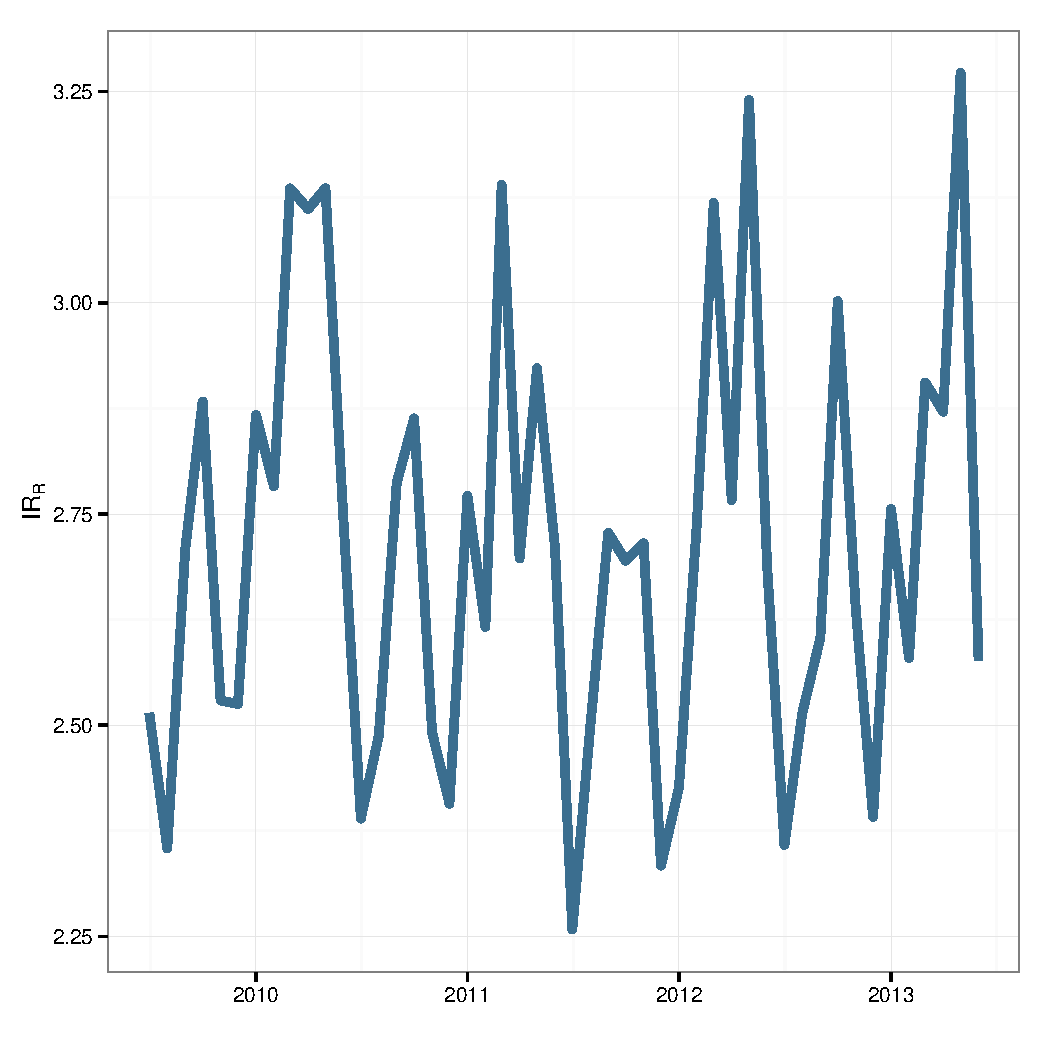
\includegraphics[width=\maxwidth]{figure/IR_S} 

}



\end{knitrout}


\paragraph{The incidence of placement into out-of-home care}

\subparagraph{Definition} The incidence of placement into out-of-home care ($IR_P$) shall be defined as the monthly total number of referrals to Children's Administration per 1,000 persons under the age of 18. This rate shall be calculated simply by 
\begin{equation}\label{eq:IRP}
IR_P = (I_P \div P_C) \cdot 1,000
\end{equation}
where $I_P$ represents the total number of placements occuring during the month and $P_C$ the number of children under the age of 18 in the general population. To the extent that estimates are available, values of $P_C$ shall be calculated from the same sources and order of priority as in $P_H$ above.

\subparagraph{SQL Code}

In this section I use a previously calculated table of interpolated values $P_C$ (\texttt{ref\_lookup\_census\_population}), a CA ``reporting layer'' table of placements into out-of-home care (\texttt{rptPlacement}), and the aforementioned (\texttt{calendar\_dim}) table.


\lstinputlisting[language=SQL]{IR_P.sql}

\subparagraph{R Code}

We plot the monthly time-series in a manner similar to what we did with $IR_R$.  


\begin{knitrout}
\definecolor{shadecolor}{rgb}{0.969, 0.969, 0.969}\color{fgcolor}\begin{kframe}
\begin{alltt}
\hlstd{dat.IR_P} \hlkwb{<-} \hlkwd{sqlQuery}\hlstd{(cn,} \hlkwd{read.sql}\hlstd{(}\hlstr{"IR_P.sql"}\hlstd{))}

\hlcom{#plot time series}
\hlkwd{ggplot}\hlstd{(dat.IR_P,} \hlkwd{aes}\hlstd{(}\hlkwc{y}\hlstd{=IR_P,} \hlkwc{x}\hlstd{=month))} \hlopt{+}
  \hlkwd{geom_line}\hlstd{(}\hlkwc{colour}\hlstd{=poc_colors[}\hlnum{1}\hlstd{],} \hlkwc{size}\hlstd{=}\hlnum{2}\hlstd{)} \hlopt{+}
  \hlkwd{labs}\hlstd{(}\hlkwc{y} \hlstd{=} \hlkwd{expression}\hlstd{(IR[P]),} \hlkwc{x} \hlstd{=} \hlstr{""}\hlstd{)} \hlopt{+}
  \hlkwd{theme_bw}\hlstd{()}
\end{alltt}
\end{kframe}

{\centering 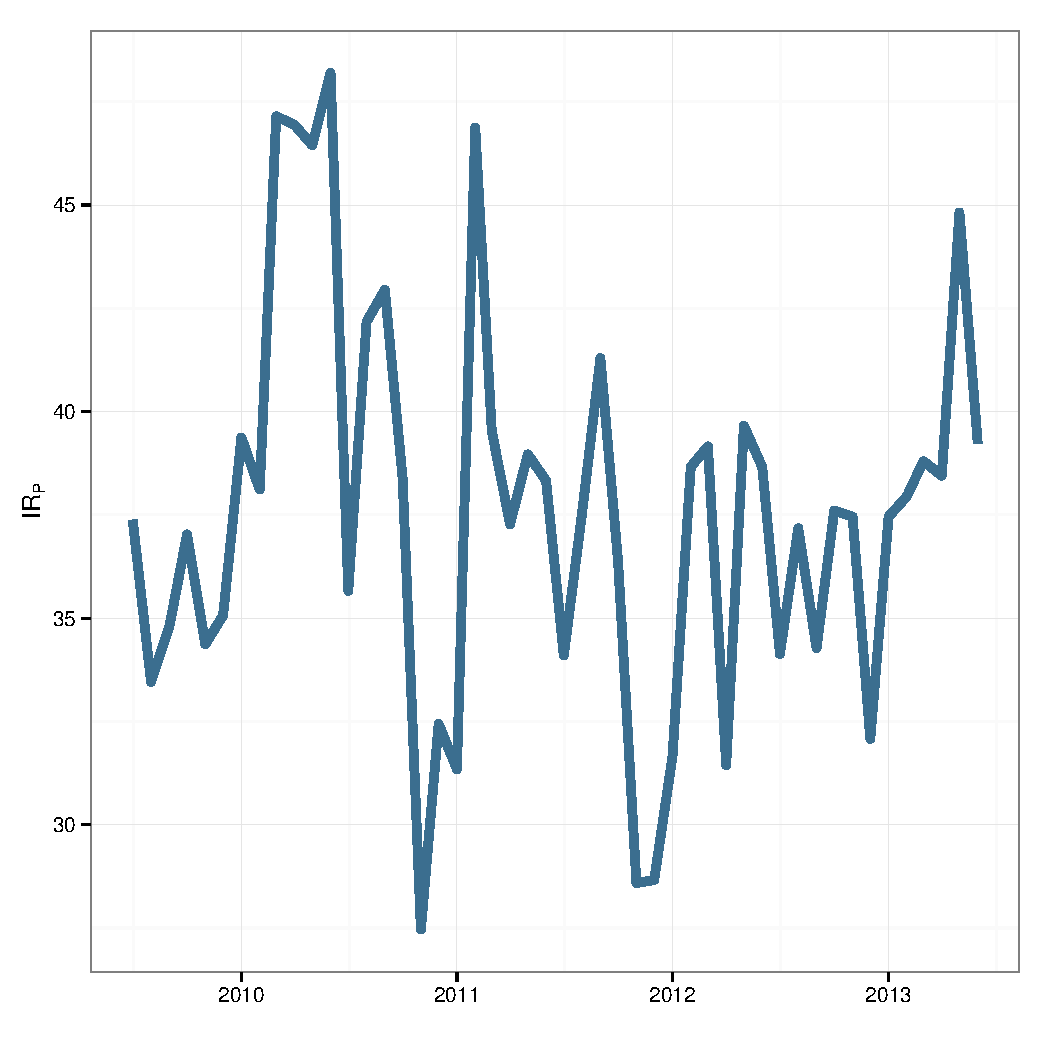
\includegraphics[width=\maxwidth]{figure/IR_P} 

}



\end{knitrout}


\paragraph{Placement rate}

\subparagraph{Definition} The rate of placement ($PR$) shall be defined as the monthly total number of first placements per 1,000 referrals to CA with no prior history of a placement in the household. For consistency with previous measurements, this measure will focus only on those referrals aledging child maltreatment or an eminent risk of serious harm to the child and will be calculated at the household level. A household is considered to have a placement if any child associated with the home on a given referral is placed into out-of-home care. This rate shall be calculated as 
\begin{equation}\label{eq:PR}
PR = (P \div I_{R_{NPP}}) \cdot 1,000
\end{equation}
where $P$ represents the total placements occuring during the month among referrals for households with no previous placement ($I_{R_{NPP}}$). 

\subparagraph{SQL Code}

The following SQL code outlines the continued use of (\texttt{tbl\_intakes}). We make use of additional fields beyond the reporting layer fields which have been calculated according to code revewed previously by CA. 

\lstinputlisting[float=h, language=SQL]{PR.sql}

Again, we plot the monthly time-series using R.  

\subparagraph{R Code}

\begin{knitrout}
\definecolor{shadecolor}{rgb}{0.969, 0.969, 0.969}\color{fgcolor}\begin{kframe}
\begin{alltt}
\hlstd{dat.PR} \hlkwb{<-} \hlkwd{sqlQuery}\hlstd{(cn,} \hlkwd{read.sql}\hlstd{(}\hlstr{"PR.sql"}\hlstd{))}

\hlcom{#plot time series}
\hlkwd{ggplot}\hlstd{(dat.PR,} \hlkwd{aes}\hlstd{(}\hlkwc{y}\hlstd{=PR,} \hlkwc{x}\hlstd{=month))} \hlopt{+}
  \hlkwd{geom_line}\hlstd{(}\hlkwc{colour}\hlstd{=poc_colors[}\hlnum{1}\hlstd{],} \hlkwc{size}\hlstd{=}\hlnum{2}\hlstd{)} \hlopt{+}
  \hlkwd{labs}\hlstd{(}\hlkwc{y} \hlstd{=} \hlkwd{expression}\hlstd{(PR),} \hlkwc{x} \hlstd{=} \hlstr{""}\hlstd{)} \hlopt{+}
  \hlkwd{theme_bw}\hlstd{()}
\end{alltt}
\end{kframe}

{\centering 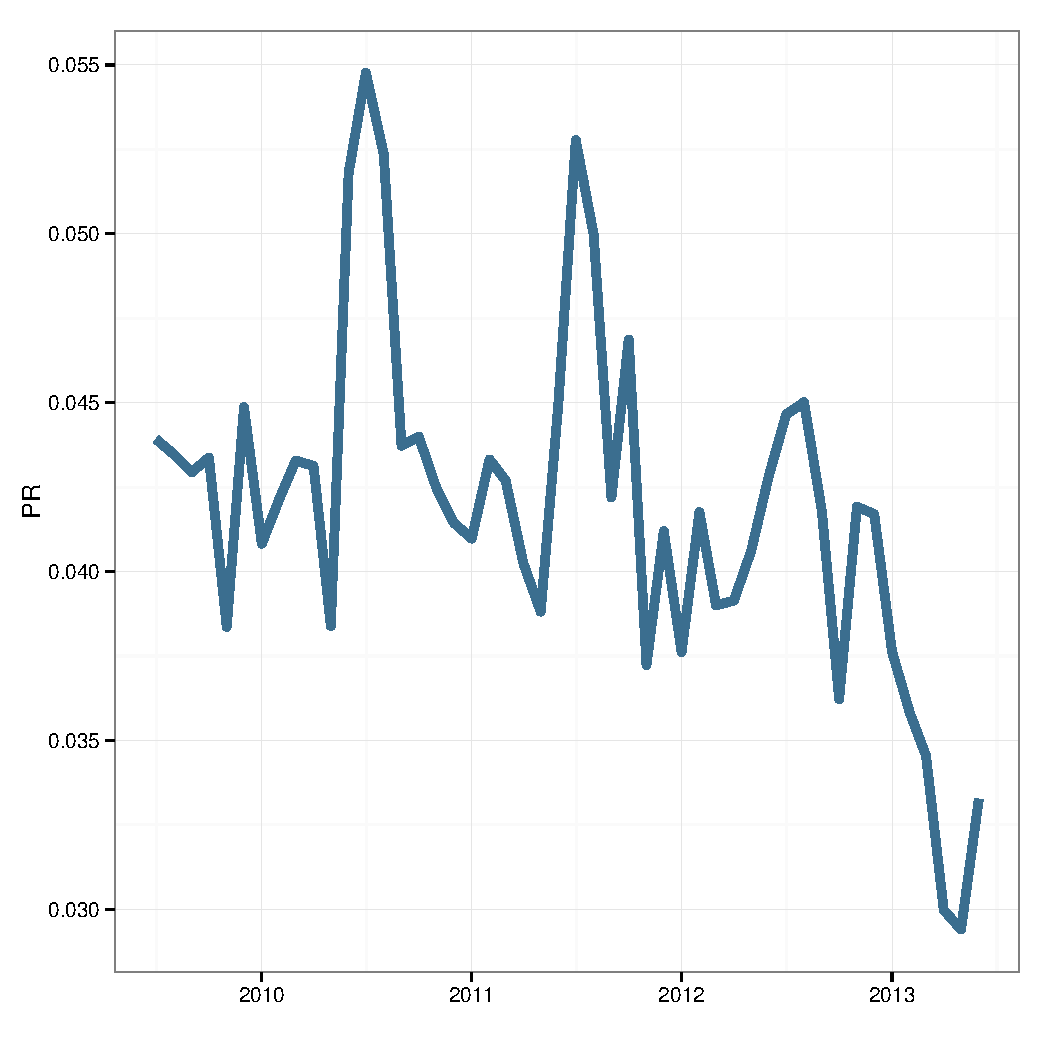
\includegraphics[width=\maxwidth]{figure/PR} 

}



\end{knitrout}



\paragraph{Finding rate}

\subparagraph{Definition} The rate of household findings ($FR$) shall be defined as the monthly total number of first findings of child-abuse or neglect per 1,000 referrals to CA with no prior history of a founded allegation of child abuse or neglect. This measure will focus only on those referrals aledging child maltreatment or an eminent risk of serious harm to the child and will be calculated at the household level. A household is considered to have a finding if any allegation from a given referral is founded. This rate shall be calculated as 
\begin{equation}\label{eq:FR}
FR = (F \div I_{R_{NPF}}) \cdot 1,000
\end{equation}
where $F$ represents the total findings occuring during the month among referrals for households with no previous finding ($I_{R_{NPF}}$). 

\subparagraph{SQL Code}

The following SQL code outlines the continued use of (\texttt{tbl\_intakes}). Here, we make use of additional fields beyond the reporting layer fields which have been calculated according to code revewed previously by CA. 

\lstinputlisting[float=h, language=SQL]{FR.sql}

Again, we plot the monthly time-series using R.  

\subparagraph{R Code}

\begin{knitrout}
\definecolor{shadecolor}{rgb}{0.969, 0.969, 0.969}\color{fgcolor}\begin{kframe}
\begin{alltt}
\hlstd{dat.FR} \hlkwb{<-} \hlkwd{sqlQuery}\hlstd{(cn,} \hlkwd{read.sql}\hlstd{(}\hlstr{"FR.sql"}\hlstd{))}

\hlcom{#plot time series}
\hlkwd{ggplot}\hlstd{(dat.FR,} \hlkwd{aes}\hlstd{(}\hlkwc{y}\hlstd{=FR,} \hlkwc{x}\hlstd{=month))} \hlopt{+}
  \hlkwd{geom_line}\hlstd{(}\hlkwc{colour}\hlstd{=poc_colors[}\hlnum{1}\hlstd{],} \hlkwc{size}\hlstd{=}\hlnum{2}\hlstd{)} \hlopt{+}
  \hlkwd{labs}\hlstd{(}\hlkwc{y} \hlstd{=} \hlkwd{expression}\hlstd{(FR),} \hlkwc{x} \hlstd{=} \hlstr{""}\hlstd{)} \hlopt{+}
  \hlkwd{theme_bw}\hlstd{()}
\end{alltt}
\end{kframe}

{\centering 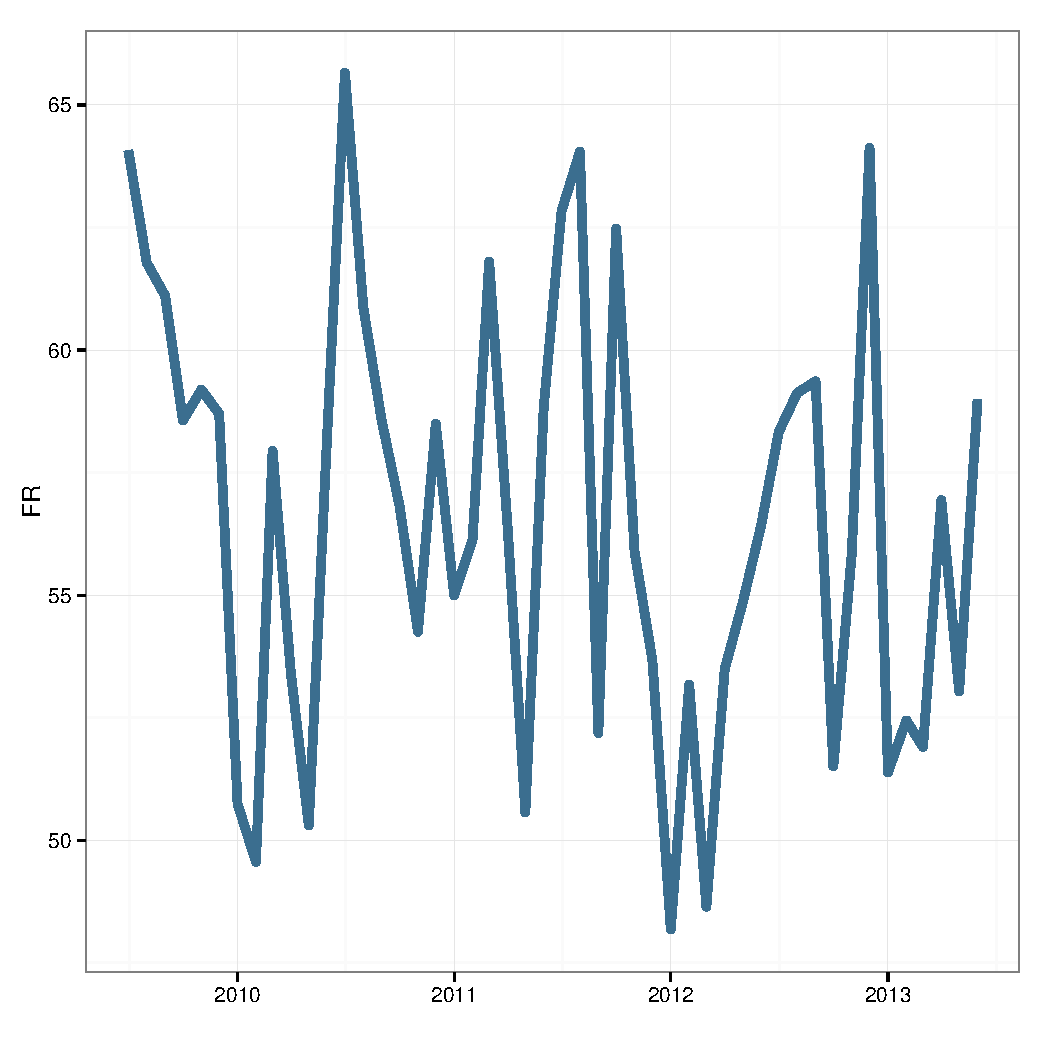
\includegraphics[width=\maxwidth]{figure/FR} 

}



\end{knitrout}



\subsubsection{Recurrence of safety concerns}

\paragraph{Order-Specific Rereferral rate} In measuring rereferrals, it is important to distinguish between first referrals ($IR_S$) and rereferrals. In general, those households that experience at least one referral to the child welfare system are at an increased risk of rereferral. As such, there is interest in distinguishing between first and higher order referrals (e.g. second referrals, third referrals, etc.). 

\subparagraph{Definition} The order-specific rereferral rate is defined as the number of referrals of a given order during a month per 1,000 households with own children under the age of 18. The formula for the first referral is given in formula ~\ref{eq:IRR}. The formula for $ith$ order rereferral rates is 
\begin{equation}\label{eq:RRRi}
RRR_i = \frac{I_{R_i}}{P_{i-1PR<18}} \cdot 1,000
\end{equation}
where $I_{R_i}$ represents the total number of $ith$ order rereferrals and $P_{i-1PR<18}$ represents the number of $ith-1$ order referrals in which all children in the household are still under the age of 18.  

\subparagraph{SQL Code}

In the following two sections of code we demonstrate the calculation of $RRR_2$ or second-order re-referrals. At this time, it is proposed that only second-order re-referrals be used as measures under 1774. Future reports may include higher-order re-referrals. In order to perform this calculation we make use of our base working table of intakes (\texttt{tbl\_intakes}), the (\texttt{calendar\_dim}), and a table of all children who appear to be associated with a given intake (\texttt{tbl\_household\_children}). For the sake of transparency, we use four seperate queries to complete this measurement: 

\begin{enumerate}
  \item A simple count of open intakes on the first day of 2010 (\texttt{RRR\_i\_start.sql}),
  \lstinputlisting[language=SQL]{RRR_i_start.sql}
  \FloatBarrier
  \item Two seperate selections give us new first intakes from 2010 to present (\texttt{RRR\_i\_entry3.sql} and \texttt{RRR\_i\_entry2.sql}), and 

  \lstinputlisting[language=SQL]{RRR_i_entry1.sql}
  \lstinputlisting[language=SQL]{RRR_i_entry2.sql}
  \item A selection of families who are ``aging-out'' of $P_{1PR<18} (\texttt{RRR\_i\_exit.sql})$
  \lstinputlisting[language=SQL]{RRR_i_exit.sql}
\end{enumerate}

\subparagraph{R Code}

The following code demonstrated how we can load these four seperate queries into R for further calculation: 

\begin{knitrout}
\definecolor{shadecolor}{rgb}{0.969, 0.969, 0.969}\color{fgcolor}\begin{kframe}
\begin{alltt}
\hlstd{dat.RRR_i.s} \hlkwb{<-} \hlkwd{sqlQuery}\hlstd{(cn,} \hlkwd{read.sql}\hlstd{(}\hlstr{"RRR_i_start.sql"}\hlstd{))}

\hlstd{dat.RRR_i.e1} \hlkwb{<-} \hlkwd{sqlQuery}\hlstd{(cn,} \hlkwd{read.sql}\hlstd{(}\hlstr{"RRR_i_entry1.sql"}\hlstd{))}

\hlstd{dat.RRR_i.e2} \hlkwb{<-} \hlkwd{sqlQuery}\hlstd{(cn,} \hlkwd{read.sql}\hlstd{(}\hlstr{"RRR_i_entry2.sql"}\hlstd{))}

\hlstd{dat.RRR_i.ex} \hlkwb{<-} \hlkwd{sqlQuery}\hlstd{(cn,} \hlkwd{read.sql}\hlstd{(}\hlstr{"RRR_i_exit.sql"}\hlstd{))}

\hlstd{P_1PRlt18} \hlkwb{<-} \hlstd{dat.RRR_i.s}\hlopt{$}\hlstd{pop_start} \hlopt{+}
  \hlstd{dat.RRR_i.e1}\hlopt{$}\hlstd{pop_enter} \hlopt{-}
  \hlstd{dat.RRR_i.ex}\hlopt{$}\hlstd{pop_exit}
\hlstd{I_R2} \hlkwb{<-} \hlstd{dat.RRR_i.e2}\hlopt{$}\hlstd{pop_enter}
\hlstd{dat.RRR_i.e2}\hlopt{$}\hlstd{RRR2} \hlkwb{<-} \hlstd{(I_R2}\hlopt{/}\hlstd{P_1PRlt18)}\hlopt{*}\hlnum{1000}


\hlcom{#plot time series}
\hlkwd{ggplot}\hlstd{(dat.RRR_i.e2,} \hlkwd{aes}\hlstd{(}\hlkwc{y}\hlstd{=RRR2,} \hlkwc{x}\hlstd{=month))} \hlopt{+}
  \hlkwd{geom_line}\hlstd{(}\hlkwc{colour}\hlstd{=poc_colors[}\hlnum{1}\hlstd{],} \hlkwc{size}\hlstd{=}\hlnum{2}\hlstd{)} \hlopt{+}
  \hlkwd{labs}\hlstd{(}\hlkwc{y} \hlstd{=} \hlkwd{expression}\hlstd{(RRR[}\hlnum{2}\hlstd{]),} \hlkwc{x} \hlstd{=} \hlstr{""}\hlstd{)} \hlopt{+}
  \hlkwd{theme_bw}\hlstd{()}
\end{alltt}
\end{kframe}

{\centering 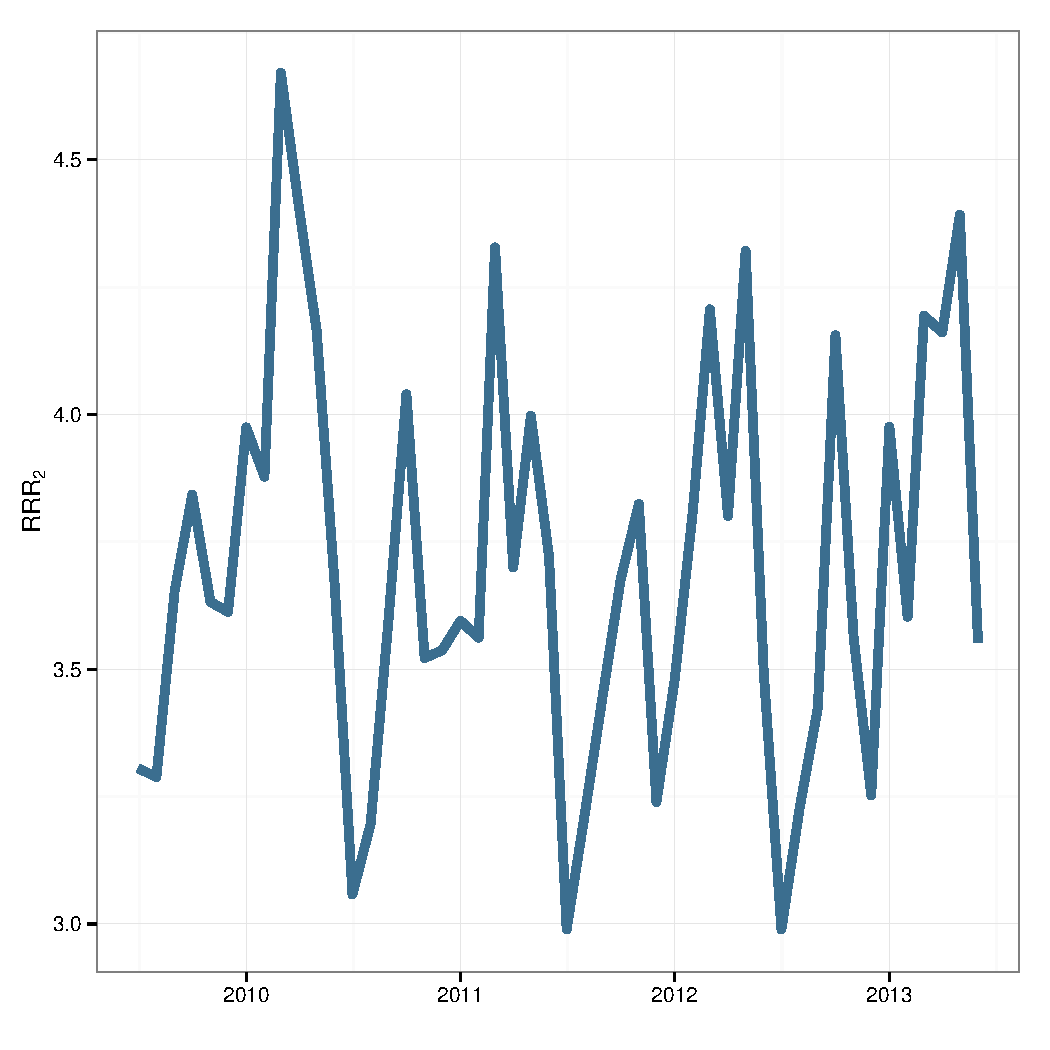
\includegraphics[width=\maxwidth]{figure/RRRi} 

}



\end{knitrout}


\paragraph{Order-Specific Refinding rate} Similarly to re-referrals, those households that experience at least one finding ($FR$) to the child welfare system are at an increased risk of refinding. As such, there is interest in distinguishing between first and higher order referrals (e.g. second referrals, third referrals, etc.). 

\subparagraph{Definition} The order-specific refinding rate is defined as the number of findings of a given order during a month per 1,000 households with own children under the age of 18 who have received $i-1$ prior referrals. The formula for the first referral is given in formula ~\ref{eq:FR}. The formula for $ith$ order rereferral rates is 
\begin{equation}\label{eq:RRRi}
RFR_i = \frac{I_{F_i}}{P_{i-1PF<18}} \cdot 1,000
\end{equation}
where $I_{F_i}$ represents the total number of $ith$ order refindings and $P_{i-1PF<18}$ represents the number of $ith-1$ order findings in which all children in the household are still under the age of 18.  

\subparagraph{SQL Code}

In the following two sections of code we demonstrate the calculation of $RFR_2$ or second-order re-finding rate. At this time, it is proposed that only second-order re-findings be used as measures under 1774. Future reports may include higher-order re-findings. Similar to $RRR_i$, we perform this calculation using our base working table of intakes (\texttt{tbl\_intakes}), (\texttt{calendar\_dim}), and a table of all children who appear to be associated with a given intake (\texttt{tbl\_household\_children}). For the sake of transparency, we again use four seperate queries to complete this measurement: 

\begin{enumerate}
  \item A simple count of open intakes on the first day of 2010 with a finding indicated (\texttt{RFR\_i\_start.sql}),
  \lstinputlisting[language=SQL]{RFR_i_start.sql}
  \item Two seperate selections give us new first findings from 2010 to present (\texttt{RFR\_i\_entry1.sql} and \texttt{RFR\_i\_entry2.sql}), and 
  \lstinputlisting[language=SQL]{RFR_i_entry1.sql}
  \lstinputlisting[language=SQL]{RFR_i_entry2.sql}
  \item A selection of families who are ``aging-out'' of $P_{1PF<18} (\texttt{RFR\_i\_exit.sql})$
  \lstinputlisting[language=SQL]{RFR_i_exit.sql}
\end{enumerate}

\subparagraph{R Code}

We again load the four seperate queries into R for further calculation: 

\begin{knitrout}
\definecolor{shadecolor}{rgb}{0.969, 0.969, 0.969}\color{fgcolor}\begin{kframe}
\begin{alltt}
\hlstd{dat.RFR_i.s} \hlkwb{<-} \hlkwd{sqlQuery}\hlstd{(cn,} \hlkwd{read.sql}\hlstd{(}\hlstr{"RFR_i_start.sql"}\hlstd{))}

\hlstd{dat.RFR_i.e1} \hlkwb{<-} \hlkwd{sqlQuery}\hlstd{(cn,} \hlkwd{read.sql}\hlstd{(}\hlstr{"RFR_i_entry1.sql"}\hlstd{))}

\hlstd{dat.RFR_i.e2} \hlkwb{<-} \hlkwd{sqlQuery}\hlstd{(cn,} \hlkwd{read.sql}\hlstd{(}\hlstr{"RFR_i_entry2.sql"}\hlstd{))}

\hlstd{dat.RFR_i.ex} \hlkwb{<-} \hlkwd{sqlQuery}\hlstd{(cn,} \hlkwd{read.sql}\hlstd{(}\hlstr{"RFR_i_exit.sql"}\hlstd{))}

\hlstd{P_1PFlt18} \hlkwb{<-} \hlstd{dat.RFR_i.s}\hlopt{$}\hlstd{pop_start} \hlopt{+}
  \hlstd{dat.RFR_i.e1}\hlopt{$}\hlstd{pop_enter} \hlopt{-}
  \hlstd{dat.RFR_i.ex}\hlopt{$}\hlstd{pop_exit}
\hlstd{I_F2} \hlkwb{<-} \hlstd{dat.RFR_i.e2}\hlopt{$}\hlstd{pop_enter}
\hlstd{dat.RFR_i.e2}\hlopt{$}\hlstd{RFR2} \hlkwb{<-} \hlstd{(I_F2}\hlopt{/}\hlstd{P_1PFlt18)}\hlopt{*}\hlnum{1000}


\hlcom{#plot time series}
\hlkwd{ggplot}\hlstd{(dat.RFR_i.e2,} \hlkwd{aes}\hlstd{(}\hlkwc{y}\hlstd{=RFR2,} \hlkwc{x}\hlstd{=month))} \hlopt{+}
  \hlkwd{geom_line}\hlstd{(}\hlkwc{colour}\hlstd{=poc_colors[}\hlnum{1}\hlstd{],} \hlkwc{size}\hlstd{=}\hlnum{2}\hlstd{)} \hlopt{+}
  \hlkwd{labs}\hlstd{(}\hlkwc{y} \hlstd{=} \hlkwd{expression}\hlstd{(RFR[}\hlnum{2}\hlstd{]),} \hlkwc{x} \hlstd{=} \hlstr{""}\hlstd{)} \hlopt{+}
  \hlkwd{theme_bw}\hlstd{()}
\end{alltt}
\end{kframe}

{\centering 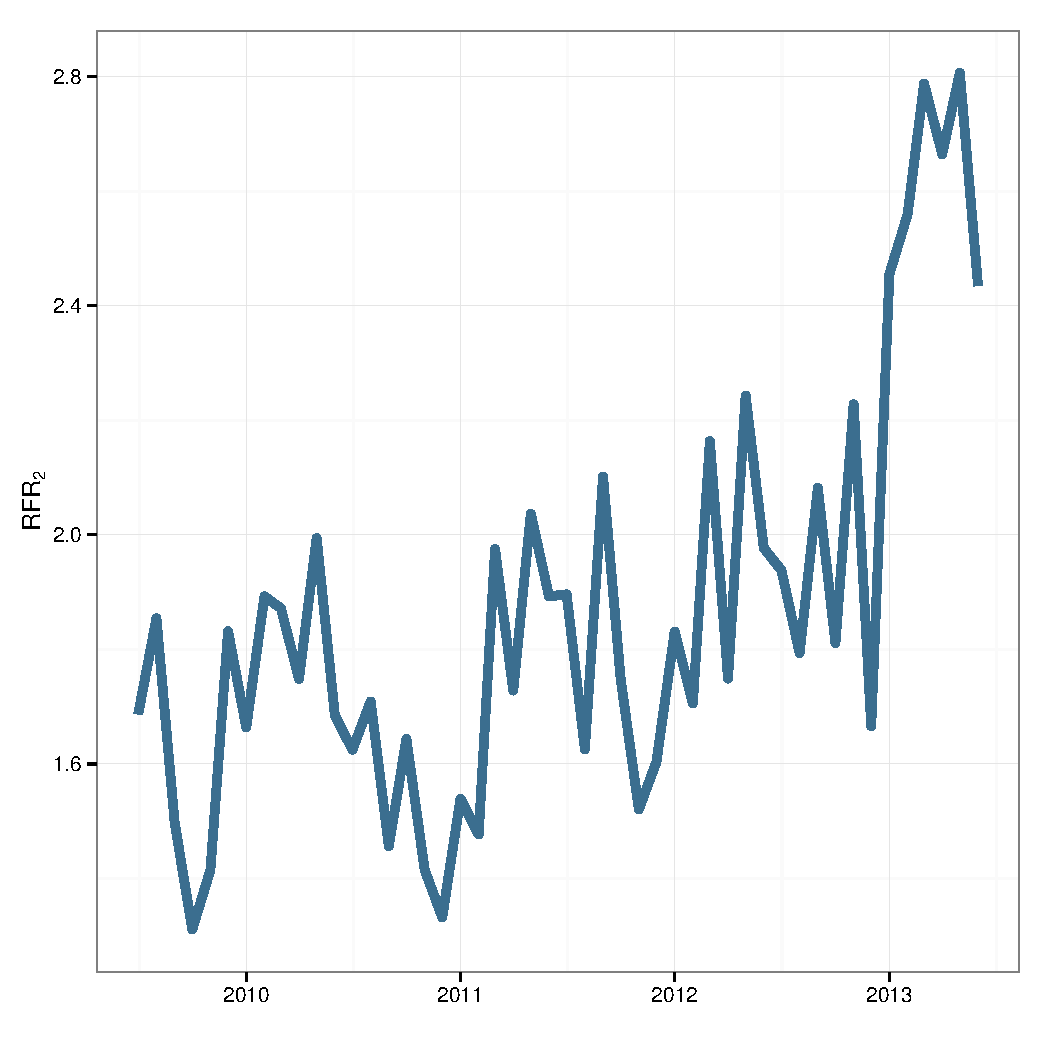
\includegraphics[width=\maxwidth]{figure/RFRi} 

}



\end{knitrout}


\paragraph{Foster-Care Finding Rate} The final safety measurement concerns the rate of findings per day of foster care. This is the first ``care-day'' measurement proposed in this document - measurements in which the denominator is a count of days of out-of-home care for some population as opposed to a count of some type of person. 

\subparagraph{Definition} The Foster-Care Finding Rate (${}_{FC}FR$) follows the newly proposed CFSR measurements where ${}_{FC}FR$ is defined as 

\begin{equation}\label{eq:_FCFR}
{}_{FC}FR = \frac{{}_{FC}I_F}{c} \cdot 100,000
\end{equation}
where $c$ represents the total number of care days provided by CA in a given year and ${}_{FC}I_F$ represents the number of maltreatment findings for children in out-of-home care over that period. This measurement excludes children in foster care for less than 8 days and also excludes reports made within the first 7 days of the referral. 

\subparagraph{SQL Code}

In the following two sections of code we demonstrate the calculation of $RRR_2$ or second-order re-referrals. For the sake of transparency and efficiency, we first load relevant data into a series of ``global'' temporary tables and then select from these tables. We plot a yearly time-series here as opposed to a monthly time-series for consistency with the CFSR measurements. 

\lstinputlisting[language=SQL]{FCFR_temp.sql}
\lstinputlisting[language=SQL]{FCFR_select.sql}


\subparagraph{R Code}

In this chunk of code, we first execute the temporary table script (hence we need not assign the results of our first query to an object) and then select from our temporary tables with the select script. We then plot the data using \texttt{ggplot2} as shown previously. 


\begin{knitrout}
\definecolor{shadecolor}{rgb}{0.969, 0.969, 0.969}\color{fgcolor}\begin{kframe}
\begin{alltt}
\hlkwd{sqlQuery}\hlstd{(cn,} \hlkwd{read.sql}\hlstd{(}\hlstr{"FCFR_temp.sql"}\hlstd{))}
\end{alltt}
\begin{verbatim}
## character(0)
\end{verbatim}
\begin{alltt}
\hlstd{dat.FCFR} \hlkwb{<-} \hlkwd{sqlQuery}\hlstd{(cn,} \hlkwd{read.sql}\hlstd{(}\hlstr{"FCFR_select.sql"}\hlstd{))}

\hlcom{#plot time series}
\hlkwd{ggplot}\hlstd{(dat.FCFR,} \hlkwd{aes}\hlstd{(}\hlkwc{y}\hlstd{=FCFR,} \hlkwc{x}\hlstd{=fiscal_yr))} \hlopt{+}
  \hlkwd{geom_line}\hlstd{(}\hlkwc{colour}\hlstd{=poc_colors[}\hlnum{1}\hlstd{],} \hlkwc{size}\hlstd{=}\hlnum{2}\hlstd{)} \hlopt{+}
  \hlkwd{labs}\hlstd{(}\hlkwc{y} \hlstd{=} \hlkwd{expression}\hlstd{(}\hlkwd{paste}\hlstd{(\{\}[FC],} \hlstr{"FR"}\hlstd{)),} \hlkwc{x} \hlstd{=} \hlstr{""}\hlstd{)} \hlopt{+}
  \hlkwd{theme_bw}\hlstd{()}
\end{alltt}
\end{kframe}

{\centering 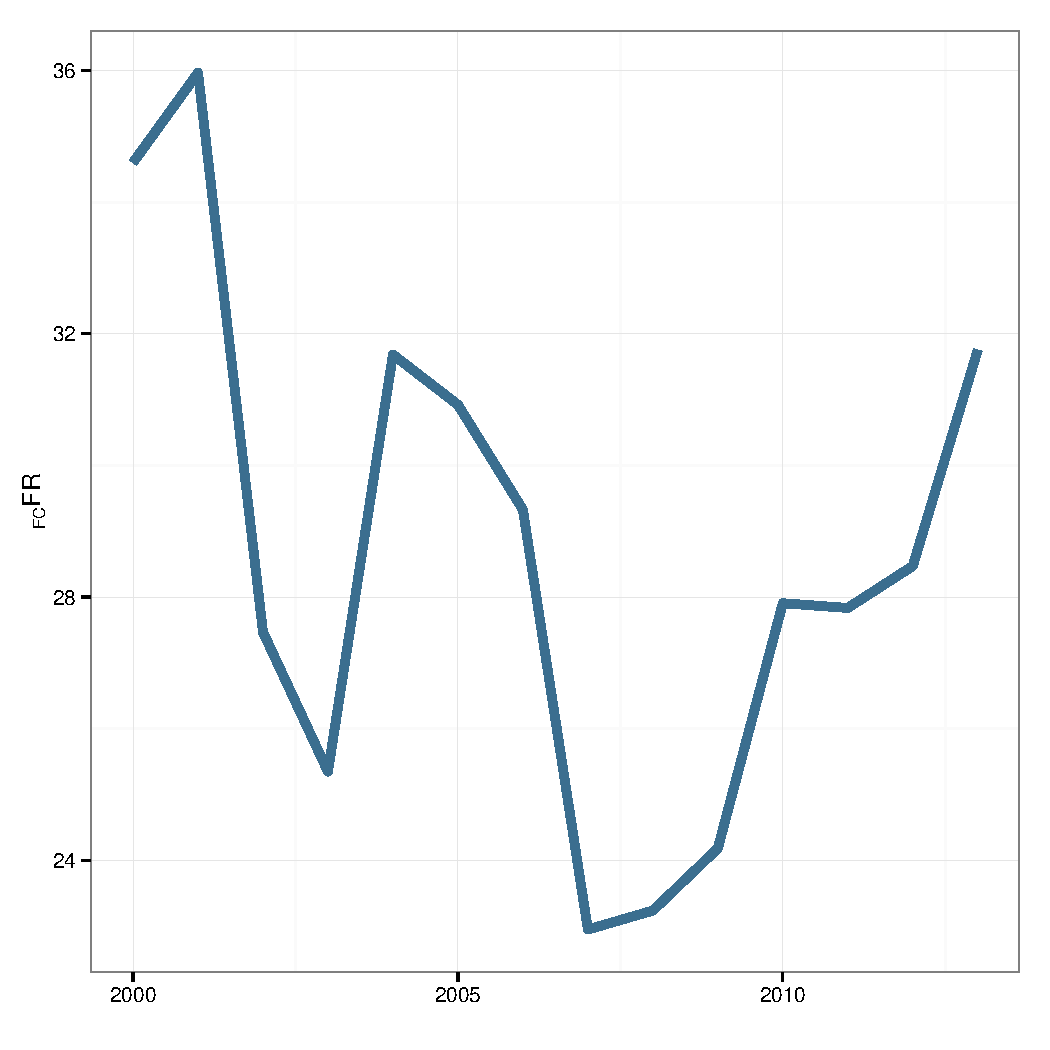
\includegraphics[width=\maxwidth]{figure/_FCFR} 

}



\end{knitrout}




\subsection{Measurements Related to Permanency}

\subsubsection{Placement stability for children placed in out-of-home care}

\paragraph{Order-specific mobility rates according to length of stay}

\paragraph{Order-transition-specific mobility rates according to length of stay}

\subsubsection{Length of time to permanence for children in out-of-home care}

\paragraph{Probability of Remaining in Care for 1 Year} This measurement is similar to the proposed CFSR measurement requiring exit to permanency within 12 months. However, instead of calculating a specific percentage, we propose that a Kaplan-Meier estimator be used to better account for right censoring of children who either age-out of the system or exit to a form of permanency other than adoption, reunification, or some form of guardianship. 
 
\subparagraph{Definition} The Kaplan-Meier estimator for a federally recognized form of permanency $P$ is given as

\begin{equation}\label{eq:KM}
{}_P\hat S(t) = \prod\limits_{t_i<t} \frac{n_i-p_{i}}{n_i}
\end{equation}
 
where $n_{i}$ is the number still in care just prior to time $t_{i}$, and $p_{i}$ is the number of permanency events at $t_{i}$. Thus, the probability of exit within 1 year is given as ${}_P\hat S(365)$. A reasonable approximation of the new CFSR measurement is given as

\begin{equation}\label{eq:KM}
(1 - {}_P\hat S(365)) \cdot 100. 
\end{equation}

\subparagraph{SQL Code}

POC is currently working on an implementation of a Kaplan-Meier estimator in SQL server. For our present purposes, however, we will select the relevant data with SQL code and calculate ${}_P\hat S(365)$ using \texttt{survival} package in R. The releveant SQL code is as follows: 

\lstinputlisting[language=SQL]{P_hat_S.sql}

\subparagraph{R Code}

The following code allows us to load the data using the aformentioned SQL script as we have done previously. We then set our model using the R syntax for event history models. This model statement indicates our time variable \texttt{t} and our permanency variable \texttt{p}. We set the model ``equal to'' \texttt{fiscal\_yr} which tells R that we want to calculate seperate survival functions for each entry-year. The fitted survival functions are assigned to an object named \texttt{fit}. We then create a new dataframe called \texttt{dat} which we initialize with a \texttt{fiscal\_yr} column indicating the fiscal year in question and a \texttt{P\_hat\_S365} colum into which we will loop values of ${}_P\hat S(365)$ for each fiscal year. 


\begin{knitrout}
\definecolor{shadecolor}{rgb}{0.969, 0.969, 0.969}\color{fgcolor}\begin{kframe}
\begin{alltt}
\hlkwd{require}\hlstd{(survival)}
\end{alltt}


{\ttfamily\noindent\itshape\color{messagecolor}{\#\# Loading required package: survival\\\#\# Loading required package: splines}}\begin{alltt}
\hlstd{dat.P_hat_S} \hlkwb{<-} \hlkwd{sqlQuery}\hlstd{(cn,} \hlkwd{read.sql}\hlstd{(}\hlstr{"p_hat_S.sql"}\hlstd{))}

\hlstd{model} \hlkwb{<-} \hlkwd{Surv}\hlstd{(t,p)} \hlopt{~} \hlstd{fiscal_yr}
\hlstd{fit} \hlkwb{<-} \hlkwd{survfit}\hlstd{(model,} \hlkwc{dat}\hlstd{=dat.P_hat_S)}

\hlstd{dat} \hlkwb{<-} \hlkwd{data.frame}\hlstd{(}\hlkwc{fiscal_yr} \hlstd{=} \hlnum{2000}\hlopt{:}\hlnum{2013}
                  \hlstd{,}\hlkwc{P_hat_S365} \hlstd{=} \hlkwd{rep}\hlstd{(}\hlnum{NA}\hlstd{,}\hlkwd{length}\hlstd{(fit}\hlopt{$}\hlstd{strata)))}
\hlkwa{for}\hlstd{(i} \hlkwa{in} \hlnum{1}\hlopt{:}\hlkwd{length}\hlstd{(fit}\hlopt{$}\hlstd{strata))\{}
  \hlstd{sum_i} \hlkwb{<-} \hlkwd{summary}\hlstd{(fit[i])}
  \hlstd{idx} \hlkwb{<-} \hlkwd{which.min}\hlstd{(}\hlkwd{abs}\hlstd{(}\hlkwd{summary}\hlstd{(fit[i])}\hlopt{$}\hlstd{time}\hlopt{-}\hlnum{365}\hlstd{))}
  \hlstd{dat}\hlopt{$}\hlstd{P_hat_S365[i]} \hlkwb{<-} \hlstd{sum_i}\hlopt{$}\hlstd{surv[idx]}
\hlstd{\}}

\hlcom{#plot time series}
\hlkwd{ggplot}\hlstd{(dat,} \hlkwd{aes}\hlstd{(}\hlkwc{y}\hlstd{=P_hat_S365,} \hlkwc{x}\hlstd{=fiscal_yr))} \hlopt{+}
  \hlkwd{geom_line}\hlstd{(}\hlkwc{colour}\hlstd{=poc_colors[}\hlnum{1}\hlstd{],} \hlkwc{size}\hlstd{=}\hlnum{2}\hlstd{)} \hlopt{+}
  \hlkwd{labs}\hlstd{(}\hlkwc{y} \hlstd{=} \hlkwd{expression}\hlstd{(}\hlkwd{paste}\hlstd{(\{\}[P]}
                            \hlstd{,}\hlkwd{hat}\hlstd{(S)}
                            \hlstd{,}\hlstr{"("}
                            \hlstd{,}\hlnum{365}
                            \hlstd{,}\hlstr{")"}\hlstd{))}
       \hlstd{,}\hlkwc{x} \hlstd{=} \hlstr{""}\hlstd{)} \hlopt{+}
  \hlkwd{theme_bw}\hlstd{()}
\end{alltt}
\end{kframe}
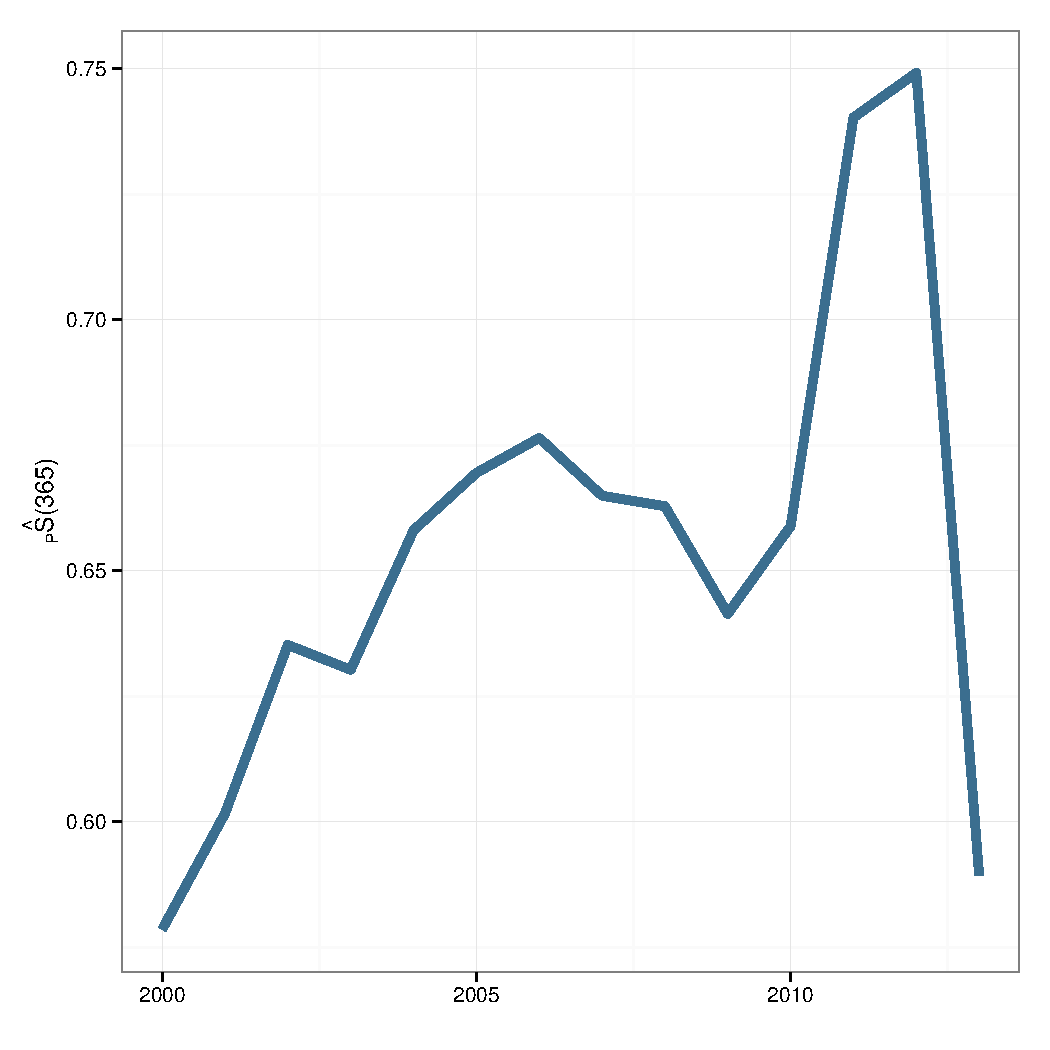
\includegraphics[width=\maxwidth]{figure/p_hat_S} 

\end{knitrout}


\begin{knitrout}
\definecolor{shadecolor}{rgb}{0.969, 0.969, 0.969}\color{fgcolor}\begin{kframe}
\begin{alltt}
\hlkwd{require}\hlstd{(survival)}
\hlstd{dat.A_hat_S} \hlkwb{<-} \hlkwd{sqlQuery}\hlstd{(cn,} \hlkwd{read.sql}\hlstd{(}\hlstr{"A_hat_S.sql"}\hlstd{))}

\hlstd{model} \hlkwb{<-} \hlkwd{Surv}\hlstd{(t,a)} \hlopt{~} \hlstd{fiscal_yr}
\hlstd{fit} \hlkwb{<-} \hlkwd{survfit}\hlstd{(model,} \hlkwc{dat}\hlstd{=dat.A_hat_S)}

\hlstd{dat} \hlkwb{<-} \hlkwd{data.frame}\hlstd{(}\hlkwc{fiscal_yr} \hlstd{=} \hlnum{2000}\hlopt{:}\hlnum{2013}
                  \hlstd{,}\hlkwc{A_hat_S365} \hlstd{=} \hlkwd{rep}\hlstd{(}\hlnum{NA}\hlstd{,}\hlkwd{length}\hlstd{(fit}\hlopt{$}\hlstd{strata)))}
\hlkwa{for}\hlstd{(i} \hlkwa{in} \hlnum{1}\hlopt{:}\hlkwd{length}\hlstd{(fit}\hlopt{$}\hlstd{strata))\{}
  \hlstd{sum_i} \hlkwb{<-} \hlkwd{summary}\hlstd{(fit[i])}
  \hlstd{idx} \hlkwb{<-} \hlkwd{which.min}\hlstd{(}\hlkwd{abs}\hlstd{(}\hlkwd{summary}\hlstd{(fit[i])}\hlopt{$}\hlstd{time}\hlopt{-}\hlnum{365}\hlstd{))}
  \hlstd{dat}\hlopt{$}\hlstd{A_hat_S365[i]} \hlkwb{<-} \hlstd{sum_i}\hlopt{$}\hlstd{surv[idx]}
\hlstd{\}}

\hlcom{#plot time series}
\hlkwd{ggplot}\hlstd{(dat,} \hlkwd{aes}\hlstd{(}\hlkwc{y}\hlstd{=A_hat_S365,} \hlkwc{x}\hlstd{=fiscal_yr))} \hlopt{+}
  \hlkwd{geom_line}\hlstd{(}\hlkwc{colour}\hlstd{=poc_colors[}\hlnum{1}\hlstd{],} \hlkwc{size}\hlstd{=}\hlnum{2}\hlstd{)} \hlopt{+}
  \hlkwd{labs}\hlstd{(}\hlkwc{y} \hlstd{=} \hlkwd{expression}\hlstd{(}\hlkwd{paste}\hlstd{(\{\}[A]}
                            \hlstd{,}\hlkwd{hat}\hlstd{(S)}
                            \hlstd{,}\hlstr{"("}
                            \hlstd{,}\hlnum{365}
                            \hlstd{,}\hlstr{")"}\hlstd{))}
       \hlstd{,}\hlkwc{x} \hlstd{=} \hlstr{""}\hlstd{)} \hlopt{+}
  \hlkwd{theme_bw}\hlstd{()}
\end{alltt}
\end{kframe}
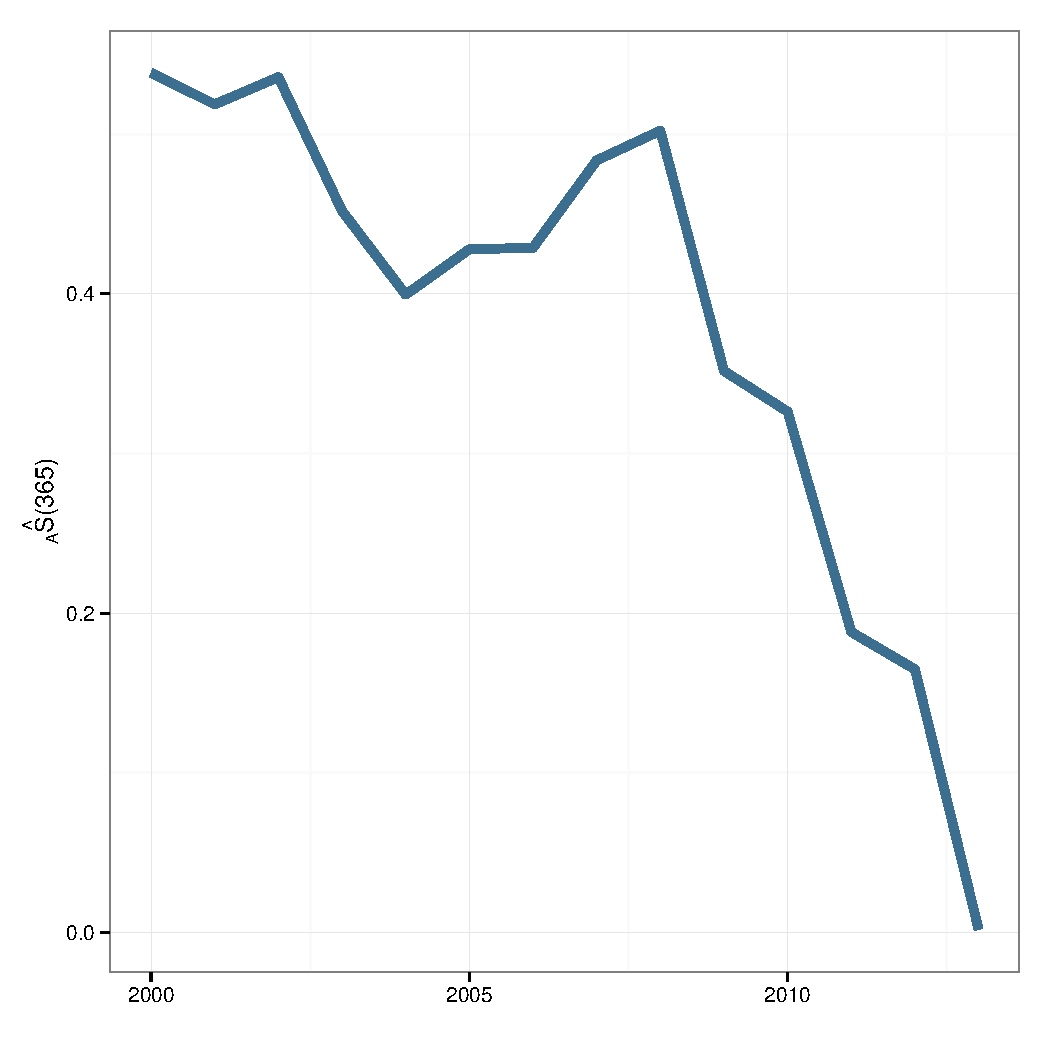
\includegraphics[width=\maxwidth]{figure/A_hat_S} 

\end{knitrout}





\subsubsection{Safe reunification of children placed in out-of-home care}
 
\paragraph{Reentry rate according to permanency duration}
 
\paragraph{Probability of Permanency for 1 Year} This measurement is similar to the proposed CFSR measurement examining reentry within 12 months. However, instead of calculating a specific percentage, we propose that a Kaplan-Meier estimator be used to better account for right censoring of children who either age-out of the system or exit to a form of permanency other than adoption, reunification, or some form of guardianship.

\subparagraph{Definition} The Kaplan-Meier estimator for reentry $R$ from a federally recognized form of permanency is given as

\begin{equation}\label{eq:KM}
{}_R\hat S(t) = \prod\limits_{t_i<t} \frac{n_i-r_{i}}{n_i}
\end{equation}
 
where $n_{i}$ is the number still in permanency just prior to time $t_{i}$, and $r_{i}$ is the number of reentry events at $t_{i}$. Thus, the probability of exit within 1 year is given as ${}_R\hat S(365)$. A reasonable approximation of the new CFSR measurement is given as

\begin{equation}\label{eq:KM}
(1 - {}_P\hat S(365)) \cdot 100. 
\end{equation}

\subparagraph{SQL Code}

As mentioned, POC is currently working on an implementation of a Kaplan-Meier estimator in SQL server. For our present purposes, however, we will select the relevant data with SQL code and calculate ${}_R\hat S(365)$ as we did for ${}_P\hat S(365)$. The releveant SQL code is as follows: 

\lstinputlisting[language=SQL]{R_hat_S.sql}

\subparagraph{R Code}

The following code allows us to load the data using the aformentioned SQL script as we have done previously. We then set our model using the R syntax for event history models. This model statement indicates our time variable \texttt{t} and our reentry variable \texttt{r}. Similar to the above, We set the model ``equal to'' \texttt{fiscal\_yr} which tells R that we want to calculate seperate survival functions for each entry-year. The fitted survival functions are assigned to an object named \texttt{fit}. We then create a new dataframe called \texttt{dat} which we initialize with a \texttt{fiscal\_yr} column indicating the fiscal year in question and a \texttt{R\_hat\_S365} colum into which we will loop values of ${}_R\hat S(365)$ for each fiscal year. 


\begin{knitrout}
\definecolor{shadecolor}{rgb}{0.969, 0.969, 0.969}\color{fgcolor}\begin{kframe}
\begin{alltt}
\hlkwd{require}\hlstd{(survival)}
\hlstd{dat.R_hat_S} \hlkwb{<-} \hlkwd{sqlQuery}\hlstd{(cn,} \hlkwd{read.sql}\hlstd{(}\hlstr{"R_hat_S.sql"}\hlstd{))}

\hlstd{model} \hlkwb{<-} \hlkwd{Surv}\hlstd{(t,r)} \hlopt{~} \hlstd{fiscal_yr}
\hlstd{fit} \hlkwb{<-} \hlkwd{survfit}\hlstd{(model,} \hlkwc{dat}\hlstd{=dat.R_hat_S)}

\hlstd{dat} \hlkwb{<-} \hlkwd{data.frame}\hlstd{(}\hlkwc{fiscal_yr} \hlstd{=} \hlnum{2000}\hlopt{:}\hlnum{2013}
                  \hlstd{,}\hlkwc{R_hat_S365} \hlstd{=} \hlkwd{rep}\hlstd{(}\hlnum{NA}\hlstd{,}\hlkwd{length}\hlstd{(fit}\hlopt{$}\hlstd{strata)))}
\hlkwa{for}\hlstd{(i} \hlkwa{in} \hlnum{1}\hlopt{:}\hlkwd{length}\hlstd{(fit}\hlopt{$}\hlstd{strata))\{}
  \hlstd{sum_i} \hlkwb{<-} \hlkwd{summary}\hlstd{(fit[i])}
  \hlstd{idx} \hlkwb{<-} \hlkwd{which.min}\hlstd{(}\hlkwd{abs}\hlstd{(}\hlkwd{summary}\hlstd{(fit[i])}\hlopt{$}\hlstd{time}\hlopt{-}\hlnum{365}\hlstd{))}
  \hlstd{dat}\hlopt{$}\hlstd{R_hat_S365[i]} \hlkwb{<-} \hlstd{sum_i}\hlopt{$}\hlstd{surv[idx]}
\hlstd{\}}

\hlcom{#plot time series}
\hlkwd{ggplot}\hlstd{(dat,} \hlkwd{aes}\hlstd{(}\hlkwc{y}\hlstd{=R_hat_S365,} \hlkwc{x}\hlstd{=fiscal_yr))} \hlopt{+}
  \hlkwd{geom_line}\hlstd{(}\hlkwc{colour}\hlstd{=poc_colors[}\hlnum{1}\hlstd{],} \hlkwc{size}\hlstd{=}\hlnum{2}\hlstd{)} \hlopt{+}
  \hlkwd{labs}\hlstd{(}\hlkwc{y} \hlstd{=} \hlkwd{expression}\hlstd{(}\hlkwd{paste}\hlstd{(\{\}[R]}
                            \hlstd{,}\hlkwd{hat}\hlstd{(S)}
                            \hlstd{,}\hlstr{"("}
                            \hlstd{,}\hlnum{365}
                            \hlstd{,}\hlstr{")"}\hlstd{))}
       \hlstd{,}\hlkwc{x} \hlstd{=} \hlstr{""}\hlstd{)} \hlopt{+}
  \hlkwd{theme_bw}\hlstd{()}
\end{alltt}
\end{kframe}
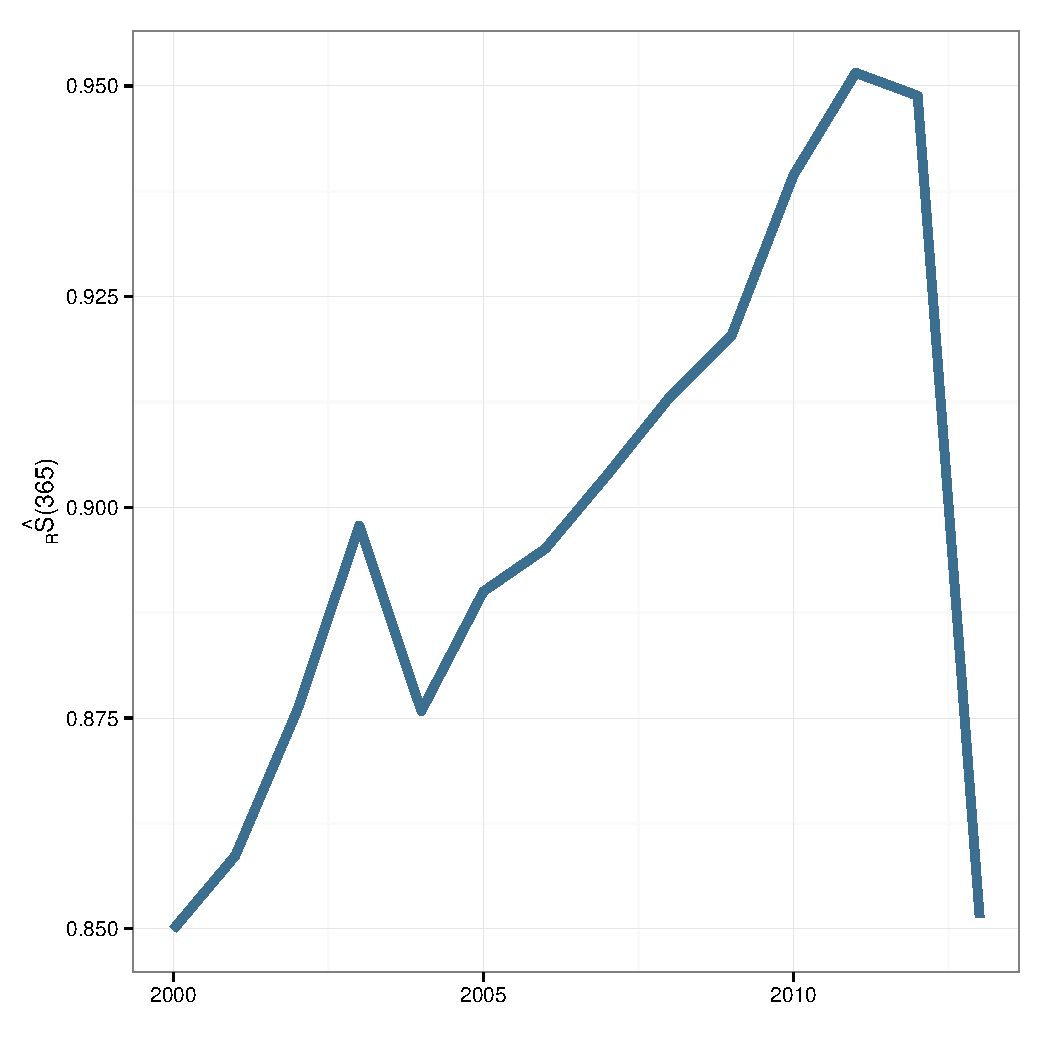
\includegraphics[width=\maxwidth]{figure/r_hat_S} 

\end{knitrout}




%\paragraph{Median Time to Permanency} 
% 
% For this sample, the estimated survival probability must never have reached 50\%, that is, the survival step function does not cross the line y=.5. The Kaplan-Meier estimate, especially since it is a non-parametric method, makes no inference about survival times (i.e., the shape of the survival function) beyond the range of times found in the data. Mean survival time, on the other hand, is a statement about the observed times. It shouldn't be taken to mean the length of time a subject can be expected to survive.
%  
% 
% \subparagraph{Definition} The median time to permanency $p$ is defined as the minimum amount of time $t_i$ that a child would need to remain in care in order to have a probability of remaining in care that was $\le 0.5$. The probability of remaining in care at a particular point in time is estimated using the survival function defined above. We thus caculate the median time to a particular form of permanency ${}_P\tilde{T}$ as 
% 
% \begin{equation}\label{eq:KM_med}
% \min(t_{i} \mid \hat {}_PS(t_{i}) \le .5 )
% \end{equation}
%  
%  
% \subparagraph{SQL Code}

% \subparagraph{SQL Code}
% 
% \FloatBarrier
% \lstinputlisting[language=SQL]{dat4.sql}
% \FloatBarrier
% 
% 

% 
% 
% model <- Surv(los,adt) ~ fiscal_yr
% fit <- survfit(model, dat=dat4[dat4$column_lbl == 'q1',])
% lt$q1a <- rep(NA,length(fit$strata))
% for(i in 1:length(fit$strata)){
%   lt$q1a[i] <- ifelse(identical(1-summary(fit[i])$surv[which.min(abs(summary(fit[i])$time-365))],numeric(0))
%                      ,NA
%                      ,1-summary(fit[i])$surv[which.min(abs(summary(fit[i])$time-365))]
%   )
%                      
% }
% 
% model <- Surv(los,gdn) ~ fiscal_yr
% fit <- survfit(model, dat=dat4[dat4$column_lbl == 'q1',])
% lt$q1g <- rep(NA,length(fit$strata))
% for(i in 1:length(fit$strata)){
%   lt$q1g[i] <- ifelse(identical(1-summary(fit[i])$surv[which.min(abs(summary(fit[i])$time-365))],numeric(0))
%                      ,NA
%                      ,1-summary(fit[i])$surv[which.min(abs(summary(fit[i])$time-365))]
%   )
%                      
% }
% 
% 
% model <- Surv(los,reu) ~ fiscal_yr
% fit <- survfit(model, dat=dat4[dat4$column_lbl == 'q2',])
% lt$q2r <- rep(NA,length(fit$strata))
% 
% for(i in 1:(length(fit$strata)-1)){
%   lt$q2r[i+1] <- ifelse(identical(1-summary(fit[i])$surv[which.min(abs(summary(fit[i])$time-365))],numeric(0))
%                      ,NA
%                      ,1-summary(fit[i])$surv[which.min(abs(summary(fit[i])$time-365))]
%   )
%                      
% }
% 
% model <- Surv(los,adt) ~ fiscal_yr
% 
% fit <- survfit(model, dat=dat4[dat4$column_lbl == 'q2',])
% lt$q1a <- rep(NA,length(fit$strata))
% for(i in 1:(length(fit$strata)-1)){
%   lt$q1a[i+1] <- ifelse(identical(1-summary(fit[i])$surv[which.min(abs(summary(fit[i])$time-365))],numeric(0))
%                      ,NA
%                      ,1-summary(fit[i])$surv[which.min(abs(summary(fit[i])$time-365))]
%   )
%                      
% }
% 
% 
% model <- Surv(los,adt) ~ fiscal_yr
% fit <- survfit(model, dat=dat4[dat4$column_lbl == 'q2',])
% lt$q2g <- rep(NA,length(fit$strata))
% 
% for(i in 1:(length(fit$strata)-1)){
%   lt$q2g[i+1] <- ifelse(identical(1-summary(fit[i])$surv[which.min(abs(summary(fit[i])$time-365))],numeric(0))
%                      ,NA
%                      ,1-summary(fit[i])$surv[which.min(abs(summary(fit[i])$time-365))]
%   )
%                      
% }
% 
% 
% 
% 
% 
% 
% model <- Surv(yr3los,yr3reu) ~ fiscal_yr
% fit <- survfit(model, dat=dat4[dat4$age_at_fy_end >= 2,])
% lt$q3r <- rep(NA,length(fit$strata))
% 
% for(i in 1:(length(fit$strata)-2)){
%   lt$q3r[i+2] <- ifelse(identical(1-summary(fit[i])$surv[which.min(abs(summary(fit[i])$time-365))],numeric(0))
%                      ,NA
%                      ,1-summary(fit[i])$surv[which.min(abs(summary(fit[i])$time-365))]
%   )
%                      
% }
% 
% model <- Surv(yr1los,yr1adt) ~ fiscal_yr
% 
% fit <- survfit(model, dat=dat4)
% lt$q1a <- rep(NA,length(fit$strata))
% for(i in 1:length(fit$strata)){
%   lt$q1a[i] <- ifelse(identical(1-summary(fit[i])$surv[which.min(abs(summary(fit[i])$time-365))],numeric(0))
%                      ,NA
%                      ,1-summary(fit[i])$surv[which.min(abs(summary(fit[i])$time-365))]
%   )
%                      
% }
% 
% 
% model <- Surv(yr2los,yr2adt) ~ fiscal_yr
% fit <- survfit(model, dat=dat4[dat4$age_at_fy_end>=1,])
% lt$q2a <- rep(NA,length(fit$strata))
% 
% for(i in 1:(length(fit$strata)-1)){
%   lt$q2a[i+1] <- ifelse(identical(1-summary(fit[i])$surv[which.min(abs(summary(fit[i])$time-365))],numeric(0))
%                      ,NA
%                      ,1-summary(fit[i])$surv[which.min(abs(summary(fit[i])$time-365))]
%   )
%                      
% }
% 
% 
% model <- Surv(yr3los,yr3adt) ~ fiscal_yr
% fit <- survfit(model, dat=dat4[dat4$age_at_fy_end >= 2,])
% lt$q3a <- rep(NA,length(fit$strata))
% 
% for(i in 1:(length(fit$strata)-2)){
%   lt$q3a[i+2] <- ifelse(identical(1-summary(fit[i])$surv[which.min(abs(summary(fit[i])$time-365))],numeric(0))
%                      ,NA
%                      ,1-summary(fit[i])$surv[which.min(abs(summary(fit[i])$time-365))]
%   )
%                      
% }
% 
% model <- Surv(yr1los,yr1gdn) ~ fiscal_yr
% 
% fit <- survfit(model, dat=dat4)
% lt$q1g <- rep(NA,length(fit$strata))
% for(i in 1:length(fit$strata)){
%   lt$q1g[i] <- ifelse(identical(1-summary(fit[i])$surv[which.min(abs(summary(fit[i])$time-365))],numeric(0))
%                      ,NA
%                      ,1-summary(fit[i])$surv[which.min(abs(summary(fit[i])$time-365))]
%   )
%                      
% }
% 
% 
% model <- Surv(yr2los,yr2gdn) ~ fiscal_yr
% fit <- survfit(model, dat=dat4[dat4$age_at_fy_end >=1,])
% lt$q2g <- rep(NA,length(fit$strata))
% 
% for(i in 1:(length(fit$strata)-1)){
%   lt$q2g[i+1] <- ifelse(identical(1-summary(fit[i])$surv[which.min(abs(summary(fit[i])$time-365))],numeric(0))
%                      ,NA
%                      ,1-summary(fit[i])$surv[which.min(abs(summary(fit[i])$time-365))]
%   )
%                      
% }
% 
% 
% model <- Surv(yr3los,yr3gdn) ~ fiscal_yr
% fit <- survfit(model, dat=dat4[dat4$age_at_fy_end >= 2,])
% lt$q3g <- rep(NA,length(fit$strata))
% 
% for(i in 1:(length(fit$strata)-2)){
%   lt$q3g[i+2] <- ifelse(identical(1-summary(fit[i])$surv[which.min(abs(summary(fit[i])$time-365))],numeric(0))
%                      ,NA
%                      ,1-summary(fit[i])$surv[which.min(abs(summary(fit[i])$time-365))]
%   )
%                      
% }
% 
% 
% 
% 
% 
% 
% fit <- survfit(model, dat=dat4[dat4$los > 365,])
% lt$q2 <- rep(0,length(fit$strata))
% 
% for(i in 1:length(fit$strata)){
%   lt$q2[i] <- ifelse(identical(1-summary(fit[i])$surv[which.min(abs(summary(fit[i])$time-365))],numeric(0))
%                      ,NA
%                      ,1-summary(fit[i])$surv[which.min(abs(summary(fit[i])$time-365))]
%   )
%                      
% }
% 
% 
% cuminc <- cuminc(ftime=dat4$los
%                 ,fstatus=dat4$fstatus
%                 ,group=dat4$fiscal_yr
%                 ,cencode=0)
% 
% model <- Surv(los,reu) ~ fiscal_yr
% fit <- survfit(model, dat=dat4)
% 
% 
% d <- matrix(nrow = 3*14, ncol = 24)
% for(j in (2000:2013)){
%   dat4 <- sqlQuery(cn, read.sql("dat4_r1.sql"))
%   start <- j-2
%   x <- start:j
%   a_x <- c(16,1,1)
%   f_x <- c(.1,.5,.1)
%   
%   model <- Surv(los,reu) ~ 1
%   srv <- start:j
%   for(i in (start:j)){
%     if(i == start){
%       fit <- survfit(model, dat=dat4[dat4$entry_yr < start & dat4$fiscal_yr == j,])
%       srv[start] <- 1-fit$surv[match(which.min(abs(fit$time-365)),fit$time)]
%     } else {
%       fit <- survfit(model, dat=dat4[dat4$entry_yr == i & dat4$fiscal_yr == j,])
%       srv[i] <- 1-fit$surv[match(which.min(abs(fit$time-365)),fit$time)]
%     }
%   }
%   nq_xr <- srv[start:j]
%   
%   model <- Surv(los,adt)~1
%   for(i in (start:j)){
%     if(i == start){
%       fit <- survfit(model, dat=dat4[dat4$entry_yr < start & dat4$fiscal_yr == j,])
%       srv[start] <- 1-fit$surv[match(which.min(abs(fit$time-365)),fit$time)]
%     } else {
%       fit <- survfit(model, dat=dat4[dat4$entry_yr == i & dat4$fiscal_yr == j,])
%       srv[i] <- 1-fit$surv[match(which.min(abs(fit$time-365)),fit$time)]
%     }
%   }
%   nq_xa <- srv[start:j]
%   
%   model <- Surv(los,gdn)~1
%   for(i in (start:j)){
%     if(i == start){
%       fit <- survfit(model, dat=dat4[dat4$entry_yr < start & dat4$fiscal_yr == j,])
%       srv[start] <- 1-fit$surv[match(which.min(abs(fit$time-365)),fit$time)]
%     } else {
%       fit <- survfit(model, dat=dat4[dat4$entry_yr == i & dat4$fiscal_yr == j,])
%       srv[i] <- 1-fit$surv[match(which.min(abs(fit$time-365)),fit$time)]
%     }
%   }
%   nq_xg <- srv[start:j]
%   
%   model <- Surv(los,oth)~1
%   for(i in (start:j)){
%     if(i == start){
%       fit <- survfit(model, dat=dat4[dat4$entry_yr < start & dat4$fiscal_yr == j,])
%       srv[start] <- 1-fit$surv[match(which.min(abs(fit$time-365)),fit$time)]
%     } else {
%       fit <- survfit(model, dat=dat4[dat4$entry_yr == i & dat4$fiscal_yr == j,])
%       srv[i] <- 1-fit$surv[match(which.min(abs(fit$time-365)),fit$time)]
%     }
%   }
%   nq_xo <- srv[start:j]
%   
%   x <- rev(x)
%   a_x <- rev(a_x)
%   f_x <- rev(f_x)
%   nq_xr <- rev(nq_xr) 
%   nq_xa <- rev(nq_xa) 
%   nq_xg <- rev(nq_xg) 
%   nq_xo <- rev(nq_xo) 
% 
%   l_0r <- sum(dat4[dat4$fiscal_yr == j,]$reu)
%   l_0a <- sum(dat4[dat4$fiscal_yr == j,]$adt)
%   l_0g <- sum(dat4[dat4$fiscal_yr == j,]$gdn)
%   l_0o <- sum(dat4[dat4$fiscal_yr == j,]$oth)
%   
%   l_0 <- (l_0r + l_0a + l_0g + l_0o)
%   
%   l_0r <- l_0r/l_0
%   l_0a <- l_0a/l_0
%   l_0g <- l_0g/l_0
%   l_0o <- l_0o/l_0
%   
%   l_0r <- l_0r*1000
%   l_0a <- l_0a*1000
%   l_0g <- l_0g*1000
%   l_0o <- l_0o*1000
%   
%   l_xr <- rep(NA, 3)
%   l_xa <- rep(NA, 3)
%   l_xg <- rep(NA, 3)
%   l_xo <- rep(NA, 3)
%   
%   l_xr[1] <- l_0r
%   l_xa[1] <- l_0a
%   l_xg[1] <- l_0g
%   l_xo[1] <- l_0o
%   
%   for(i in 1:2){
%     l_xr[i+1] <- (1-nq_xr[i])*l_xr[i]
%     l_xa[i+1] <- (1-nq_xa[i])*l_xa[i]
%     l_xg[i+1] <- (1-nq_xg[i])*l_xg[i]
%     l_xo[i+1] <- (1-nq_xo[i])*l_xo[i]  
%   }
%   
%   L_xr <- rep(NA, 3)
%   L_xa <- rep(NA, 3)
%   L_xg <- rep(NA, 3)
%   L_xo <- rep(NA, 3)
%   
%   for(i in (1:3)){
%     if(i == 3){
%       L_xr[i] <- a_x*f_x*l_xr[i]
%       L_xa[i] <- a_x*f_x*l_xa[i]
%       L_xg[i] <- a_x*f_x*l_xg[i]
%       L_xo[i] <- a_x*f_x*l_xo[i]
%     } else {
%       L_xr[i] <- a_x*(f_x*l_xr[i] + (1-f_x)*l_xr[i+1])
%       L_xa[i] <- a_x*(f_x*l_xa[i] + (1-f_x)*l_xa[i+1])
%       L_xg[i] <- a_x*(f_x*l_xg[i] + (1-f_x)*l_xg[i+1])
%       L_xo[i] <- a_x*(f_x*l_xo[i] + (1-f_x)*l_xo[i+1])
%     }
%   }
%   
%   T_xr <- rev(cumsum(L_xr))
%   T_xa <- rev(cumsum(L_xa))
%   T_xg <- rev(cumsum(L_xg))
%   T_xo <- rev(cumsum(L_xo))
%   
%   e_xr <- T_xr/l_xr
%   e_xa <- T_xa/l_xa
%   e_xg <- T_xg/l_xg
%   e_xo <- T_xo/l_xo
%   
% dp <- cbind(j, x, a_x, f_x
%                        ,nq_xr, nq_xa, nq_xg, nq_xo
%                        ,l_xr, l_xa, l_xg, l_xo
%                        ,L_xr, L_xa, L_xg, L_xo
%                        ,T_xr, T_xa, T_xg, T_xo
%                        ,e_xr, e_xa, e_xg, e_xo)
% row_from <- 3*j-5999
% row_to <- 3*j-5997
% d[row_from:row_to,1:24] <- dp
% 
% }
% @
% 
% \paragraph{Average Time to Permanency}
% 
% \subparagraph{Definition} 
% 
% \subparagraph{SQL Code}
% 
% \subparagraph{R Code}
% 
% \subsubsection{Safe reunification of children placed in out-of-home care}
% 
% \paragraph{Reentry rate according to permanency duration}
% 
% \paragraph{Outcome-specific-reentry rate according to permanency duration}
% 
% \subsubsection{Timely adoptions}
% 
% \paragraph{Adoption-rate according to legally free duration}
% 
% \subsection{Measurements related to well-being}
% 
% \subsubsection{Maintenance of family relationships}
% 
% \paragraph{Prevelance of sibling groups placed together}
% 
% \subsubsection{Adolescent well-being in placement}
% 
% \paragraph{Age-specific AWOL rate among according to AWOL history}
% 
% \subsubsection{Levels of educational readiness and attainment for children served by the child welfare system}
% 
% \paragraph{Third-grade reading proficiency ratio for foster children}
% 
% \paragraph{Kindergarten-readiness ratio for foster children}
% 
% \paragraph{Prevelance of post-secondary planning activities for foster children}
% 
% \subsubsection{Adult functioning of youth who have aged out of the child welfare system, including social integration and independence}
% 
% \paragraph{Age-specific cummulative grade attainment ratio for former foster children}
% 
% \paragraph{Age-specific median years of schooling for former foster children}



\end{document}
